\documentclass[10pt]{article}
\usepackage{fullpage}
\renewcommand{\baselinestretch}{1.08}

\usepackage{amsthm,amsfonts,amssymb,mathrsfs,amsmath,latexsym,mathtools}
\usepackage{cite}
\usepackage{epsfig}
\usepackage{float}
\usepackage{graphicx}
\usepackage{hyperref}
\usepackage{comment}
\usepackage{enumerate}
\usepackage[shortlabels]{enumitem}
\usepackage{enumitem}
\usepackage{caption}
\usepackage{subcaption}
\usepackage{overpic}
\usepackage[super]{nth}
\usepackage{bbm}


%%%%%%%%%%%%%%%%%%%%%%%%     author defined     %%%%%%%%%%%%%%%%%%%%%%%%%
\usepackage{tikz}

\theoremstyle{plain}
\newtheorem{theorem}{Theorem}[section]
\newtheorem{lemma}[theorem]{Lemma}
\theoremstyle{definition}
\newtheorem{example}[theorem]{Example}
\newtheorem{remark}[theorem]{Remark}

\newcommand{\beq}{ \begin{equation} }
\newcommand{\eeq}{ \end{equation} }
\newcommand{\beqq}{ \begin{equation*} }
\newcommand{\eeqq}{ \end{equation*} }

%%%%%%%%%%%%%%%%%%%%%%%%%%%%%%%%%%%%%%%%%%%%%%%%%%%%%%%%%%%%%

\newcommand{\dd}{\mathrm{d}}
\newcommand{\ii}{\mathrm{i}}
\newcommand{\R}{\mathbb{R}}
\newcommand{\compC}{\mathbb{C}}
\newcommand{\Z}{\mathbb{Z}}
\newcommand{\Prob}{\mathrm{P}}    %{\mathbb{P}}  

\newcommand{\pkmath}{\mathsf}  %%%%     PKPZ math font 
\newcommand{\pkFdist}{F^{\mathrm{pKPZ}}} %\mathfrak{F}} %%%%   PKPZ  distribution function F  
\newcommand{\pkDdisc}{\mathfrak{D}}  %%%%     PKPZ  D for dist function
\newcommand{\pkCdisc}{C}  %%%%     PKPZ  C for dist function
\newcommand{\pkt}{\tau} %%%%     PKPZ time \tau   
\newcommand{\pkga}{\gamma} %%%%     PKPZ location \gamma when \frac{\gamma}{2} 
\newcommand{\pkh}{\pkmath{h}}  %%%%     PKPZ height h 
\newcommand{\pkheight}{\mathbf{h}}  
\newcommand{\ptap}{x}  %%%%     PTASEP height h 
\newcommand{\ptat}{t}  %%%%     PTASEP height h 
\newcommand{\ptah}{h}  %%%%     PTASEP height h 
\newcommand{\pK}{\pkmath{K}}  %%%%     PKPZ K
\newcommand{\pid}{\pkmath{1}}  %%%%     PKPZ id operator 
\newcommand{\pspace}{\pkmath{S}}  %%%%     PKPZ space 


\newcommand{\kmath}{\mathsf}  %%%%     KPZ math font 
\newcommand{\kFdist}{F} %%%%   KPZ  distribution function F  
\newcommand{\kDdisc}{\mathfrak{D}}  %%%%     KPZ  D for dist function
\newcommand{\kCdisc}{\mathfrak{C}}  %%%%     KPZ  C for dist function
\newcommand{\kt}{\tau} %%%%     KPZ time \tau   
\newcommand{\kga}{\gamma} %%%%     KPZ location \gamma when \frac{\gamma}{2} 
\newcommand{\kh}{\kmath{h}}  %%%%     KPZ height h 
\newcommand{\kheight}{\mathbf{h}} %{\mathcal{H}}  
\newcommand{\tap}{k}  %%%%     TASEP height h 
\newcommand{\tat}{t}  %%%%     TASEP height h 
\newcommand{\tah}{h}  %%%%     TASEP height h 
\newcommand{\kid}{\kmath{1}}  %%%%     KPZ id operator 
\newcommand{\kK}{\kmath{K}}  %%%%     KPZ K
%\newcommand{\ku}{\kmath{u}}  %%%%     KPZ u
%\newcommand{\kv}{\kmath{v}}  %%%%     KPZ v
\newcommand{\ku}{u}  %%%%     KPZ u
\newcommand{\kv}{v}  %%%%     KPZ v
\newcommand{\ka}{\kmath{a}}  %%%%     KPZ a
\newcommand{\kb}{\kmath{b}}  %%%%     KPZ b
\newcommand{\kD}{\kmath{D}}  %%%%     KPZ D
\newcommand{\kM}{\kmath{M}}  %%%%     KPZ M
\newcommand{\kp}{\kmath{p}}  %%%%     KPZ p
\newcommand{\kr}{\kmath{r}}  %%%%     KPZ r
\newcommand{\knt}{\kmath{t}}  %%%%     KPZ t
\newcommand{\kny}{\kmath{y}}  %%%%     KPZ y
\newcommand{\knx}{\kmath{x}}  %%%%     KPZ x

\newcommand{\pE}{\mathrm{E}}  %%%%     Poisson DLPP E
\newcommand{\pL}{\mathrm{L}}  %%%%     Poisson DLPP L

\newcommand{\TW}{\mathrm{TW}}  %%%%     TW
\newcommand{\FTW}{\mathrm{F}_{\TW}}  %%%%     F_TW
\newcommand{\diag}{\mathrm{diag}}  %%%%     diag


%%%%%%%%%%%%%%%%%%%%%%%%%%%%%%%%%%%%%%%%%%%%%%%%%%%%%%%%%%%%%


% To include the section number in the equation numbering:
\numberwithin{equation}{section}

%%%%%%%%%%%%%%%%%%%%%%%%%%%%%%%%%%%%%%%%%%%%%%%%%%%%%
\title{KPZ limit theorems}

%\title{Integrable structure for the multipoint distributions KPZ fixed point}

\author{Jinho Baik\footnote{Department of Mathematics, University of Michigan,
Ann Arbor, MI, 48109, USA, \texttt{baik@umich.edu}}}

\date \today %{September 1, 2021}

%%%%%%%%%%%%%%%%%%%%%%%%%%%%%%%%%%%%%%%%%%%%%%%%%

\begin{document}

\maketitle

\begin{abstract}
One-dimensional interacting particle systems, 1+1 random growth models, and two-dimensional directed polymers define 2d height fields.
The KPZ universality conjecture posits that an appropriately scaled height function converges to a model-independent universal random field for a large class of models. 
We survey limit theorems for a few models and discuss changes that arise in different domains. 
In particular, we present recent results on periodic domains. 
We also comment on integrable probability models, integrable differential equations, and universality. 
\end{abstract}

%\setcounter{tocdepth}{1}
%\tableofcontents


%%%%%%%%%%%%%%%%%%%%%%%%%%%%%%%%%%%%%%%%%%%%%%%%%%%%%%%%%%%%%
\section{Introduction}

%Over the last two decades exciting progresses occurred regarding the KPZ universality. 

The KPZ universality is concerned with, among others, one-dimensional interacting particle systems, 1+1 random growth, and two-dimensional directed polymers. 
These models define height functions $\kheight(x, t)$, two-dimensional random fields, where $x$ represents the one-dimensional spatial position and $t$ the time.  
A height function encodes the integrated current for interacting particle systems, the height for random growth models, and the free energy for directed polymer models. See Section \ref{sec:TASEP} for an example. 
The KPZ universality conjecture is that for a large class of models, the scaled height function 
\beq \label{eq:heightscaled}
	\kheight_T(\gamma, \tau)= \frac{\kheight(\gamma T^{2/3}, \tau T) - c(T)}{T^{1/3}}
\eeq
converges, up to scaling factors, to a model-independent universal 2d random field, which is called the KPZ fixed point. 
Here $c(T)$ is a non-random term determined by the macroscopic limit of the height function. 
Since the height, position, and time scale as $T^{1/3}, T^{2/3}$, and $T$, respectively, 
we say that \eqref{eq:heightscaled} is a 1:2:3 scaled height function. 
We also say that a KPZ limit theorem holds if a 1:2:3 scaled height function converges in any suitable sense for the problem at hand. %in distribution. 

%Since the height, position, and time scale as $T^{1/3}, T^{2/3}$, and $T$, respectively, we say that \eqref{eq:heightscaled} is 1:2:3 scaled. 
%We also say that a KPZ limit theorem holds if a 1:2:3 scaled height function \eqref{eq:heightscaled} converges in distribution. 

Several physics papers \cite{Kardar-Parisi-Zhang86, Forster-Nelson-Stephen77, vanBeijeren-Kutner-Spohn85, Huse-Henley85} conjectured the 1:2:3 scale for various models in the mid-1980s. 
One of them is the paper \cite{Kardar-Parisi-Zhang86} of Kardar, Parisi, and Zhang on a nonlinear stochastic partial differential equation, now called the KPZ equation, from which the term KPZ universality is derived. 
These papers were followed by extensive research in the physics community. 
However, it remained unknown, even on a conjectural level, what the limit should be. 
%these physics papers was not able to give a clue to what the limit, the KPZ fixed point, should be. 

%Hence, there are two questions, one on proving the KPZ limit theorem for a large class of models and the other on determining the limit. 
%Hence, the big question is which models converge to the KPZ fixed point and what is the KPZ fixed point. 

The situation changed in 1999 with the publication of the paper \cite{Baik-Deift-Johansson99} by 
Baik, Deift, and Johansson, in which the authors considered the longest increasing subsequence problem of random permutations. 
%This problem is equivalent to the last passage time of a two-dimensional last passage percolation model, which itself is the zero-temperature version of a directed polymer model. 
This problem is equivalent to the zero-temperature free energy of a directed polymer model. 
%the last passage time of a two-dimensional last passage percolation model, which itself is the zero-temperature version of a directed polymer model. 
The paper proved that the one-point distribution of an analog of the height function converges in distribution. 
See Theorem \ref{thm:Poisson} below. 
Moreover, the authors found the limiting distribution explicitly, which turned out to be the Tracy-Widom distribution from random matrix theory. 
This connection between the KPZ universality and random matrix theory was completely unexpected at that time. 
%Hence, a one-point KPZ limit theorem was proved for one model and the limit was computed exa relationship with random matrix theory was found. 
%Soon after, Johansson \cite{Johansson00}  proved a similar result for another model, the totally asymmetric simple exclusion process, giving another example of a KPZ limit theorem. 
Soon after, Johansson \cite{Johansson00}  proved a similar result for another model, giving yet another example of a KPZ limit theorem. 
%Soon after, Johansson \cite{Johansson00}  proved a similar result for another model, the totally asymmetric simple exclusion process, %%with the step initial condition, 
%giving another example of a KPZ limit theorem. 

Exciting developments on KPZ limit theorems followed these results during the next two decades. 
%Exciting developments on KPZ limit theorems followed these breakthroughs during the next two decades. 
%There results kickstarted exciting developments on KPZ limit theorems followed these breakthroughs during the next two decades. 
For example, one-point limit theorems were extended to equal-time, multi-position distributions, multi-time distributions, and even to the 2d fields. 
Results were also generalized to several, mostly isolated, models, and algebraic underpinning of these specific models was studied. 
The 2d field limit, the KPZ fixed point, was determined, and various properties of the limit were established. 
%In terms of the spaces for the models, 
Limit theorems were also proved for infinite space, half-infinite space, and recently finite space with periodic boundary condition. 

%This article gives a historical overview of some KPZ limit theorems and presents new results on the periodic domain case. Along the way, we discuss a few topics, including integrable models, integrable differential equations, and universality. 
In this article, we give a historical overview of some KPZ limit theorems and present new results on the periodic domain case.
%In this article, we overview some KPZ limit theorems and present new results on the periodic domain case. Along the way, we discuss a few topics, including integrable models, integrable differential equations, and universality. 
We start by introducing the subjects of KPZ universality, interacting particle systems, random growth, and directed polymers, in Section \ref{sec:TASEP}, focusing on one particular example. 
Then, we discuss some limit theorems on infinite spaces in Section \ref{sec:one}-\ref{sec:multitime}. 
After briefly discussing the half-infinite space case in Section \ref{sec:half}, we present new results on the periodic case in Section \ref{sec:ring}.
Section \ref{sec:dfformula} compares the formulas of the limiting multi-point distributions for infinite and periodic cases, and Section \ref{sec:integrableDE} concerns differential equations associated with distribution functions. 
We conclude the article with some comments on universality in Section \ref{sec:univ}. 


The research on the KPZ universality has been developing rapidly and extensively over the last two decades.  
Hence, what is discussed in this article is only a small selection of the activities. 
The reader may benefit from other excellent survey articles such as \cite{Corwin11, Quastel12, Borodin-Gorin16} to see other aspects. 


%%%%%%%%%%%%%%%%%%%%%%%%%%%%%%%%%%%%%%%%%%%%%%%%%%%%%%%%%%%%%
\section{TASEP, corner growth model, and exponential DLPP} \label{sec:TASEP}

%The KPZ universality concerns with interacting particle systems, random growth, and directed polymers. 
This section discusses one of the most well-studied examples of one-dimensional interacting particle systems, 1+1 random growth, and two-dimensional directed polymers. %This example is one of the most well-studied. %This section discusses one example that has interpretations in one-dimensional interacting particle systems, 1+1 random growth, and two-dimensional directed polymers. 

%all three interpretations and illustrate how these three models are related. 


\subsection{TASEP} 

The totally asymmetric simple exclusion process (TASEP), introduced by Spitzer \cite{Spitzer70} in 1970, is a continuous-time Markov process on $\Z$. 
At any given time, each integer site of $\Z$ is occupied by at most one particle. 
A particle moves to the adjacent site to its right after a random waiting time, but only if it is empty. The waiting time is exponentially distributed of mean $1$, and the clock starts once the neighboring site becomes vacant. 
All waiting times are independent of each other. 
Note that all moves are to the right (hence, totally asymmetric),  particles can move only one step at a time (simple), and no two particles occupy the same site at the same time (exclusion). 
Figure \ref{fig:TASEP} is an example of the configuration at a particular time. 
Black dots denote particles, and white dots mark empty sites. 
In this configuration, only three particles can move, and they do so independently of each other. 

%It can be thought of as a model for moving cars on a one-lane, one-way road. 
%Consider the integer lattice $\Z$.  

\begin{figure}\centering
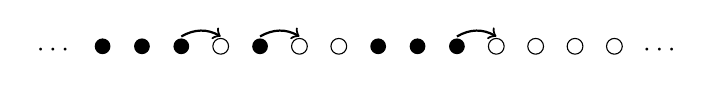
\begin{tikzpicture}[scale=0.5]
\node at (-9.2, -0.1)  {$\cdots$};
\fill (-8, 0) circle(0.2);
\fill (-7, 0) circle(0.2);
\fill (-6, 0) circle(0.2);
\draw (-5, 0) circle(0.2);
\fill (-4, 0) circle(0.2);
\draw (-3, 0) circle(0.2);
\draw (-2, 0) circle(0.2);
\fill (-1, 0) circle(0.2);
\fill (0, 0) circle(0.2);
\fill (1, 0) circle(0.2);
\draw (2, 0) circle(0.2);
\draw (3, 0) circle(0.2);
\draw (4, 0) circle(0.2);
\draw (5, 0) circle(0.2);
\node at (6.2, -0.1)  {$\cdots$};
\draw[thick, ->] (-6, 0.25) to[bend left] (-5, 0.25);
\draw[thick, ->] (-4, 0.25) to[bend left] (-3, 0.25);
\draw[thick, ->] (1, 0.25) to[bend left] (2, 0.25);
\end{tikzpicture}
\caption{TASEP}
\label{fig:TASEP}
\end{figure}


The TASEP is an example of interacting particle systems. General systems may allow, for example, left moves in addition to right moves, multi-range moves, or several particles at each site. 

One particular initial condition we focus on in this article is the step initial condition that the sites in $\Z_-\cup\{0\}$ are occupied, and all sites in $\Z_+$ are empty. 
The leftmost picture in Figure \ref{fig:corner} shows the step initial condition. 

%%%%%%%%%%%%%%%%%%%%%%%%%%%%%%%%%%%%%%%%%%%%%%%%%%%%%%%%%%%%%
\subsection{Corner growth model}

The configuration space for the TASEP is $\{0,1\}^{\Z}$ where $1$ represents the presence of a particle and $0$ an empty site. 
To each configuration, we can associate a zig-zag graph in $\R^2$ as in Figure \ref{fig:corner}. 
We assign a particle to a line segment of length $\sqrt{2}$ and slope $-1$, and an empty site to a line segment of the same length and slope $1$. 
Juxtaposing the line segments, we obtain a zig-zag graph as in Figure \ref{fig:corner}.
We call the graph a height function $\kheight:\R\to \R$ for the configuration of the TASEP, and it is unique up to translations. 
The leftmost picture in Figure \ref{fig:corner} is a translation of $\kheight(x)=|x|$, and it corresponds to the step initial condition. 

The TASEP induces a stochastic evolution of the height function, $\kheight(x,t)$, in which  
local valleys (corners) change to local peaks independently with rate $1$. 
The resulting 1+1 random growth process defined by the height function is called the corner growth process. 
See Figure \ref{fig:cornersim} for a simulation. 

%If we fix the height function for the initial condition of the TASEP, for example, by setting $\kheight(0)=0$, then t
%The TASEP induces a stochastic evolution of the height function, $\kheight(x,t)$, and it defines a 1+1 random growth process called the corner growth process. 
%In this process, local valleys (corners) change to local peaks independently of other valleys with rate $1$. 
%Some other examples of 1+1 random growth models are ballistic deposition and the KPZ equation.
%See the left picture of Figure \ref{fig:hbar} for a simulation. % of the corner growth model. 


 
\begin{figure}
\centering
\begin{minipage}{.3\textwidth}
\centering
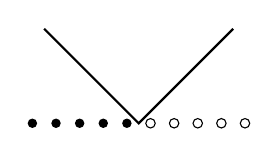
\begin{tikzpicture}[scale=0.3]
\fill (-4, 0) circle(0.2);
\fill (-3, 0) circle(0.2);
\fill (-2, 0) circle(0.2);
\fill (-1, 0) circle(0.2);
\fill (0, 0) circle(0.2);
\draw (1, 0) circle(0.2);
\draw (2, 0) circle(0.2);
\draw (3, 0) circle(0.2);
\draw (4, 0) circle(0.2);
\draw (5, 0) circle(0.2);
\draw[thick, -] (-3.5,4) -- (0.5,0) -- (4.5,4);
\end{tikzpicture}
\end{minipage}
\begin{minipage}{.3\textwidth}
\centering
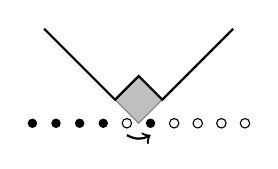
\begin{tikzpicture}[scale=0.3]
\fill (-4, 0) circle(0.2);
\fill (-3, 0) circle(0.2);
\fill (-2, 0) circle(0.2);
\fill (-1, 0) circle(0.2);
\draw (0, 0) circle(0.2);
\fill (1, 0) circle(0.2);
\draw (2, 0) circle(0.2);
\draw (3, 0) circle(0.2);
\draw (4, 0) circle(0.2);
\draw (5, 0) circle(0.2);
%\draw[thin] (-3.5,4)  -- (0.5,0) -- (4.5,4);
\fill[lightgray] (-0.5,1) -- (0.5,2) -- (1.5,1) -- (0.5, 0) -- (-0.5, 1);
\draw[thin, gray] (-0.5,1) -- (0.5,2) -- (1.5,1) -- (0.5, 0) -- (-0.5, 1);
\draw[thick, ->] (0, -0.5) to[bend right] (1, -0.5);
\draw[thick, -] (-3.5,4)  -- (-0.5,1) -- (0.5,2) -- (1.5,1) -- (4.5,4);
\end{tikzpicture}
\end{minipage}
\begin{minipage}{.3\textwidth}
\centering
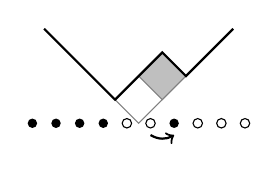
\begin{tikzpicture}[scale=0.3]
\fill (-4, 0) circle(0.2);
\fill (-3, 0) circle(0.2);
\fill (-2, 0) circle(0.2);
\fill (-1, 0) circle(0.2);
\draw (0, 0) circle(0.2);
\draw (1, 0) circle(0.2);
\fill (2, 0) circle(0.2);
\draw (3, 0) circle(0.2);
\draw (4, 0) circle(0.2);
\draw (5, 0) circle(0.2);
\draw[thin, gray] (-3.5,4)  -- (0.5,0) -- (4.5,4);
%\draw (-0.5,1) -- (0.5,2) -- (1.5,1);
\fill[lightgray] (0.5,2) -- (1.5,3) -- (2.5, 2) -- (1.5, 1) -- (0.5, 2);
\draw[thin, gray] (0.5,2) -- (1.5,3) -- (2.5, 2) -- (1.5, 1) -- (0.5, 2);
\draw[thick, ->] (1, -0.5) to[bend right] (2, -0.5);
\draw[thick, -] (-3.5,4)  -- (-0.5,1) -- (1.5,3) -- (2.5,2) -- (4.5,4);
\end{tikzpicture}
\end{minipage}
\caption{Corner growth model}
\label{fig:corner}
\end{figure}

%%%%%%%%%%%%%%%%%%%%%%%%%%%%%%%%%%%%%%%%%%%%%%%%%%%%%%%%%%%%%
\subsection{Exponential DLPP} \label{sec:DLPP}

Consider the two-dimensional lattice $\Z_+^2$. Let $(m,n)\in \Z_+^2$. 
An up/right (i.e., directed) path from $(1,1)$ to $(m,n)$ is a sequence $p=(p_i)_{i=1}^{m+n-1}$, where $p_i\in \Z_+^2$, $p_1=(1,1)$,  $p_{m+n-1}=(m,n)$, and $p_{i+1}-p_i\in \{(1,0), (0,1)\}$. 
The thick lines in Figure \ref{fig:ExpDLPP} are an example of a path in which we connected neighboring integer sites for visual aid. 
Let $w_s$, $s\in \Z_+^2$, be a collection of independent random variables. 
The normalized free energy of the directed polymer measure, introduced by Huse and Henley \cite{Huse-Henley85}, is 
\beqq
	F(m,n; \beta)= \frac1{\beta} \log \Big( \sum_{p} e^{\beta E(p)} \Big) \quad  \text{where $E(p)= \sum_{i=1}^{m+n-1} w_{p_i}$, }
\eeqq
the sum is over all directed paths $p$ from $(1,1)$ to $(m,n)$, and $\beta>0$ is the inverse temperature. 
The zero-temperature, $\beta=\infty$, case is called the directed last passage percolation (DLPP). 
In this case, the normalized free energy becomes 
\beqq
	L(m,n)= \max_{p} E(p), %\qquad  \text{where $E(p)= \sum_{i=1}^{m+n-1} w(p_i)$}
\eeqq
which we call the last passage time, interpreting $E(p)$ as the travel time using path $p$. 
%We often call it a ``point-to-point'' last passage time to differentiate from ``line-to-point'' or ``line-to-line'' last passage times in which an endpoint of a path is allowed to be any point on a line instead of being a fixed point. 

\begin{figure}
\centering
\begin{minipage}{.4\textwidth}
\centering
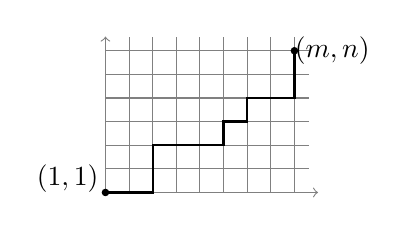
\begin{tikzpicture}[scale=0.6]
\draw [->, thin][gray] (0,0) to (4.5,0);
\draw [->, thin][gray] (0,0) to (0, 3.3);
\draw [-, thin, gray] (0,0.5) to (4.3,0.5);
\draw [-, thin, gray] (0,1) to (4.3,1);
\draw [-, thin, gray] (0,1.5) to (4.3,1.5);
\draw [-, thin, gray] (0,2) to (4.3,2);
\draw [-, thin, gray] (0,2.5) to (4.3,2.5);
\draw [-, thin, gray] (0,3) to (4.3,3);
\draw [-, thin, gray] (0.5,0) to (0.5,3.3);
\draw [-, thin, gray] (1,0) to (1,3.3);
\draw [-, thin, gray] (1.5,0) to (1.5,3.3);
\draw [-, thin, gray] (2,0) to (2,3.3);
\draw [-, thin, gray] (2.5,0) to (2.5,3.3);
\draw [-, thin, gray] (3,0) to (3,3.3);
\draw [-, thin, gray] (3.5,0) to (3.5,3.3);
\draw [-, thin, gray] (4,0) to (4,3.3);
\draw [-, thick] (0,0) to (1,0) to (1,1) to (2.5, 1) to (2.5, 1.5) to (3,1.5) to (3,2) to (4,2) to (4,3);
\fill (0,0) circle(0.08);
\fill (4,3) circle(0.08);
\node at (-0.8, 0.3)  {$(1,1)$};
\node at (4.8, 3.0)  {$(m,n)$};
\end{tikzpicture}
\caption{Exponential DLPP}
\label{fig:ExpDLPP}
\end{minipage}
\qquad 
\begin{minipage}{.4\textwidth}
\centering
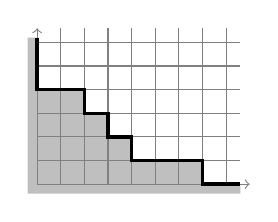
\begin{tikzpicture}[scale=0.6]
\fill[lightgray] (0, 3.1) to (0,2) to (1, 2) to (1, 1.5) to (1.5, 1.5) to (1.5, 1) to (2, 1) to (2, 0.5) to (3.5, 0.5) to (3.5, 0) to (4.3, 0) to (4.3, -0.2) to (-0.2, -0.2) to (-0.2, 3.1) to (0, 3.1);
\draw [->, thin][gray] (0,0) to (4.5,0);
\draw [->, thin][gray] (0,0) to (0, 3.3);
\draw [-, thin, gray] (0,0.5) to (4.3,0.5);
\draw [-, thin, gray] (0,1) to (4.3,1);
\draw [-, thin, gray] (0,1.5) to (4.3,1.5);
\draw [-, thin, gray] (0,2) to (4.3,2);
\draw [-, thin, gray] (0,2.5) to (4.3,2.5);
\draw [-, thin, gray] (0,3) to (4.3,3);
\draw [-, thin, gray] (0.5,0) to (0.5,3.3);
\draw [-, thin, gray] (1,0) to (1,3.3);
\draw [-, thin, gray] (1.5,0) to (1.5,3.3);
\draw [-, thin, gray] (2,0) to (2,3.3);
\draw [-, thin, gray] (2.5,0) to (2.5,3.3);
\draw [-, thin, gray] (3,0) to (3,3.3);
\draw [-, thin, gray] (3.5,0) to (3.5,3.3);
\draw [-, thin, gray] (4,0) to (4,3.3);
\draw [-, very thick] (0, 3.1) to (0,2) to (1, 2) to (1, 1.5) to (1.5, 1.5) to (1.5, 1) to (2, 1) to (2, 0.5) to (3.5, 0.5) to (3.5, 0) to (4.3, 0);
\end{tikzpicture}
\caption{An example of $G_t$}
\label{fig:ExpDLPPdual}
\end{minipage}
\end{figure}


For the case when $w_s\ge 0$, the DLPP is related to a random growth model. 
For $t>0$, define the subset of $\R^2$ by 
\beqq
	G_t= \bigcup_{s\in S_t} ( (0,1]^2+s)  \qquad 
	\text{where $S_t= \{(m, n)\in  \Z^2: L(m,n)\le t\}$}
\eeqq
and we set $L(m,n)=0$ if $m\le 0$ or $n\le 0$. See Figure \ref{fig:ExpDLPPdual}. 
Since $L(m,n)$ is greater than or equal to both $L(m-1, n)$ and $L(m, n-1)$,  
we see that if $(m,n)\in G_t$, then both points $(m-1, n)$ and $(m,n-1)$ are in $G_t$. 
The set $G_t$ grows with time $t$. 
If we regard $G_t$ in the first quadrant as a stack of boxes, we can add a new box only at the corners. %only the corners can grow. 


A special case is the exponential DLPP in which $w_s$ are exponentially distributed with mean $1$. 
In this case, each corner of $G_t$ grows independently of rate $1$, i.e., a unit box can be added to each corner independent at rate $1$.  
Thus, the boundary of $G_t$ is a rotation of the height function of the corner growth process. 
More precisely, for the TASEP with the step initial condition and the exponential DLPP, 
\beq \label{eq:heightandDLPP}
	\kheight (m-n, t )\ge m+n \quad \text{ if and only if } \quad L(m,n)\le t .
\eeq
If the TASEP starts with a different initial condition, we need to consider the exponential DLPP on a subset of $\Z^2$, determined by the initial condition. 


%%%%%%%%%%%%%%%%%%%%%%%%%%%%%%%%%%%%%%%%%%%%%%%%%%%%%%%%%%%%%
\subsection{Hydrodynamic limit and KPZ limit}

The hydrodynamic limit of TASEP is about $\kheight(x,t)$ when $x$ and $t$ are proportional. 
For the step initial condition, $\kheight(x,0)=|x|$, Rost \cite{Rost81} showed in 1981 that 
\beqq
	\frac{\kheight(xT, tT)}{T}  \to \bar{\kheight}(x,t) 
\eeqq
almost surely as $T\to \infty$, where $\bar{\kheight}(x,t) = \frac{t^2+x^2}{2t}$ for $|x|\le t$ and $\bar{\kheight}(x,t) = |x|$ for $|x|\ge t$. 
See Figure \ref{fig:hbar} for the graph. 
The hydrodynamic limit $\bar{\kheight}$ is deterministic, and it solves Burger's equation \cite{Liggett85, Liggett99}.




The KPZ limit is about the next term, $\kheight(xT, tT)- \bar{\kheight}(x,t)T$. 
Setting $x=0$ for convenience and following the 1:2:3 scale, the KPZ universality conjecture suggests that 
\beqq
	\frac{\kheight(\gamma T^{2/3}, \tau T)- \bar{\kheight}(0,\tau)T}{T^{1/3}}
\eeqq  
converges to a 2d random field. 
If we do not set $x=0$, then we should consider $\kheight(xT+ \gamma T^{2/3}, \tau T)- \bar{\kheight}(x,\tau)T$ in the numerator. 
The limiting 2d field, the KPZ fixed point, depends on the initial condition. The step initial condition for the TASEP becomes the so-called narrow wedge initial condition for the KPZ fixed point. 

\begin{figure}
\centering
\begin{minipage}{.4\textwidth}
\centering
	\centering\includegraphics[scale=0.14]{Growth.pdf}  
\caption{Simulation of the corner growth model}
\label{fig:cornersim}
\end{minipage}
\qquad 
\begin{minipage}{.4\textwidth}
\centering
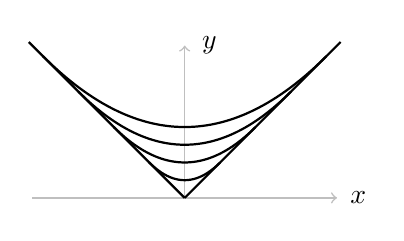
\begin{tikzpicture}[scale=0.45]
\draw [line width=0.2mm,lightgray, ->] (-4.3,0)--(4.3,0);
\draw [line width=0.2mm,lightgray, ->] (0,0)--(0,4.3);
\node at (4.9, 0) {$x$};
\node at (0.7, 4.3) {$y$};
\draw[domain=-1:1,smooth,variable=\x, thick]  plot ({\x} , {(1+\x*\x)/(2*1)});
\draw[domain=-2:2,smooth,variable=\x, thick]  plot ({\x} , {(2^2+\x*\x)/(2*2)});
\draw[domain=-3:3,smooth,variable=\x, thick]  plot ({\x} , {(3^2+\x*\x)/(2*3)});
\draw[domain=-4:4,smooth,variable=\x, thick]  plot ({\x} , {(4^2+\x*\x)/(2*4)});
\draw[domain= 0:4.4,smooth,variable=\x, thick]  plot ({\x} , {\x});
\draw[domain= -4.4:0,smooth,variable=\x, thick]  plot ({\x} , {-\x});
\end{tikzpicture}
\caption{$y= \bar{\kheight}(x, t)$ for a few values of $t$} 
\label{fig:hbar}
\end{minipage}
\end{figure}


TASEP has interpretations as an interacting particle system, a random growth process, and a last passage percolation model. 
Each of these interpretations has natural extensions and generalizations. 
The KPZ universality conjecture is that a large class of models in these generalizations has a universal limit.  
The exact class is not known, but for random growth models, three key features seem to be the locality of growth, some smoothing mechanism, and lateral growths. 
For directed last passage percolation, the universality is expected for all random variables $w_s$ with enough moments and without a large atom at the top of the support of the distribution. The last condition is to prevent the situation that there is always a path connecting $(1,1)$ and $(m,n)$ using only the top value, making the last passage time too concentrated. 

 %%%%%%%%%%%%%%%%%%%%%%%%%%%%%%%%%%%%%%%%%%%%%%%%%%%%%%%%%%%%%
\section{One-point distribution} \label{sec:one}

We discuss one-point KPZ limit theorems from \cite{Baik-Deift-Johansson99} and \cite{Johansson00} mentioned in the introduction, and extensions to other models. 

%%%%%%%%%%%%%%%%%%%%%%%%%%%%%%%%%%%%%%%%%%%%%%%%%%%%%%%%%%%%%
\subsection{Poisson DLPP}

Poisson directed last passage percolation is a variation of the exponential DLPP. 
Consider a realization of a 2d Poisson process in $\R_+^2$. 
An up/right path $p$ this time is defined as the graph of a continuous piecewise linear function of positive slopes connecting Poisson points, as shown in Figure \ref{fig:PoissonDLPP}. 
Let $\pE(p)$ denote the number of the Poisson points on $p$. 
For $(t, s)\in \R_+^2$, define
\beqq
	\pL(t,s) = \sup_{p} \pE(p), 
\eeqq
where the supremum is taken over all up/right paths $p$ from $(0,0)$ to $(t,s)$.
The next theorem follows from \cite{Baik-Deift-Johansson99}. 
The main theorem of \cite{Baik-Deift-Johansson99} is stated for the case of a fixed number of points, 
but the paper proves the Poisson points case first, from which the main theorem follows. 
Since $\pL(t,s) \stackrel{d}{=} \pL(\sqrt{ts}, \sqrt{ts})$, the next result applies to general points $(t,s)$. 

%The following is the limit theorem for one-point distribution function. 


\begin{theorem}[\cite{Baik-Deift-Johansson99}] \label{thm:Poisson}
For every $x\in \R$, 
\beqq
%	\lim_{t,s\to\infty} \frac{\pL(t,s)-2\sqrt{ts}}{(ts)^{1/6}} =^d  \TW , \qquad
	\lim_{t\to\infty} \Prob\left( \frac{\pL(t,t)-2t}{t^{1/3}}\le x \right) = \FTW (x)
\eeqq
where $\FTW$ is the Tracy-Widom distribution. 
\end{theorem}

The $1/3$-power in $t^{1/3}$ is consistent with the height scale of the KPZ universality: see \eqref{eq:heightandDLPP}. 
This result shows that the one-point marginal of the KPZ fixed point (for the narrow wedge initial condition) must be distributed as the Tracy-Widom distribution. 
The Tracy-Widom distribution is the limiting distribution of the largest eigenvalue of random Hermitian matrices such as Gaussian unitary ensemble matrices \cite{Tracy-Widom94}. 
The connection of the KPZ fixed point and random matrix theory was surprising and unexpected. See Section \ref{sec:TASEPRM} for more on this connection. 
%The fact that the limit is the Tracy-Widom distribution was surprising and unexpected. 
%Hence, the above result shows that the one-point marginal of the KPZ fixed point (for step initial condition) is r


%At the time that the above paper appeared, there was no conjecture on the limiting distribution in physics papers. 
%What turned out is that the limit is given by the Tracy--Widom distribution $\FTW$ which is the limiting distribution of the largest eigenvalue of random Hermitian matrices. 
%The surprising connection to random matrix theory was completely unanticipated at that time. 
%Poisson DLPP also has random growth interpretation - PNG model [cite]. 

\begin{figure}
\centering 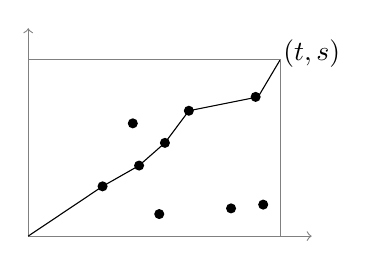
\begin{tikzpicture}[scale=0.8]
\draw [->, thin, gray] (0,0) to (4.5,0);
\draw [->, thin, gray] (0,0) to (0, 3.3);
%\fill (1.98, 3.02) circle(0.08);
\fill (1.18, 0.79) circle(0.08);
\fill (1.66, 1.79) circle(0.08);
\fill (1.76, 1.12) circle(0.08);
\fill (2.08, 0.35) circle(0.08);
\fill (2.17, 1.48) circle(0.08);
\fill (2.55, 1.99) circle(0.08);
\fill (3.22, 0.44) circle(0.08);
\fill (3.61, 2.21) circle(0.08);
\fill (3.73, 0.50) circle(0.08);
%\fill (1.89, 3.66) circle(0.1);
%\fill (3.92, 3.72) circle(0.1);
\draw [-, thin] (0,0) to (1.18, 0.79) to (1.76, 1.12) to (2.17, 1.48) to (2.55, 1.99) to (3.65, 2.21) to (4,2.8);
\draw [-, thin, gray] (4,0) to (4, 2.8) to (0, 2.8);
\node at (4.5, 2.9)  {$(t,s)$};
\end{tikzpicture}
\caption{Poisson DLPP}
\label{fig:PoissonDLPP}
\end{figure}


%%%%%%%%%%%%%%%%%%%%%%%%%%%%%%%%%%%%%%%%%%%%%%%%%%%%%%%%%%%%%
\subsection{Longest increasing subsequence}

The Poisson DLPP is particularly interesting due to its connection to longest increasing subsequences of random permutations. 
Note that finitely many points in a rectangle with distinct $x$ and $y$ coordinates can be associated with a permutation by considering the relative orderings of the coordinates. 
%Note that finitely many points in a rectangle whose $x$ and $y$ coordinates are all different can be associated with a permutation by considering the relative orderings of the coordinates. 
For example, the points in Figure \ref{fig:PoissonDLPP} are associated with the permutation $\pi=475168293$. 
For this permutation, the subsequence $45689$ is an increasing subsequence.  
Furthermore, it is the longest increasing subsequence, and its length, $5$, is equal to the last passage time $L(t,s)$. 

Let $\ell_N$ denote the length of longest increasing subsequences of a uniformly random permutation of size $N$. 
%Let $\ell_N(\pi)$ denote the length of longest increasing subsequences of the permutation $\pi$ of size $N$. 
%Consider the uniform probability measure on the set of permutations of size $N$. 
Then, $L(t,s)$ has the same distribution as $\ell_N$, where $N$ is a Poisson random variable of mean $ts$. 
Using this connection, Theorem \ref{thm:Poisson} implies, after a de-Poissonization argument, that 
$\frac{\ell_N- 2\sqrt{N}}{N^{1/6}}$ converges in distribution to the Tracy--Widom distribution. 


The problem of determining the large $N$ behavior of $\ell_N$ has a long history. The existence of the almost sure limit of $\ell_N/\sqrt{N}$ was proved by Hammersley in \cite{Hammersley72} using Kingman's ergodic subadditivity theorem. 
The fact that the limit is $2$, known as Ulam's problem, %which is equivalent to the limit $\frac{L(t,s)}{\sqrt{ts}} \to 2$ 
was proved independently by two famous papers of Ver\v{s}ik --Kerov \cite{Vershik-Kerov77} and Logan--Shepp \cite{Logan-Shepp77} in 1977. 
%The limiting distribution and the variance of $\ell_N$, which is of order $N^{2/3}$, was unknown until 
However, the limiting distribution and the variance (which is of order $N^{2/3}$) remained an open problem until the work \cite{Baik-Deift-Johansson99}. 
%The result of \cite{Baik-Deift-Johansson99} proved the limit theorem and the authors also proved that the variance of $\ell_N$ is of order $N^{2/3}$. 
Interested readers are encouraged to consult \cite{Aldous-Diaconis99, Stanley07, Romik15, Baik-Deift-Suidan}.  

%[As one can imagine, there is an interesting underlying algebraic structure behind the Poisson DLPP. It is the RS correspondence and Schur measure. See below?]

%%%%%%%%%%%%%%%%%%%%%%%%%%%%%%%%%%%%%%%%%%%%%%%%%%%%%%%%%%%%%
\subsection{Exponential DLPP}

Soon after Theorem \ref{thm:Poisson} was proved, Johansson showed that the exponential DLPP model also satisfies a similar limit theorem \cite{Johansson00}. 
We state the result in terms of the height function of the TASEP. 

\begin{theorem}[\cite{Johansson00}] \label{thm:Johansson}
Assume the step initial condition for the TASEP. 
%Set 
%\beqq
%	\tap =\kga T^{2/3}  , \qquad  \tat = 2 \kt T , \qquad	\tah= \frac{\tat}2  - T^{1/3} \kh
%\eeqq
Then, for every $( \kt, \kga, \kh) \in \R_+\times \R \times \R$, %Then, 
\beqq
%	\lim_{T\to \infty} \Prob \left(  \kheight(\tat, \tap)\le \tah \right) 
	\lim_{T\to \infty} \Prob \left(  \frac{\kheight(\kga T^{2/3}, 2 \kt T) - \tau T}{-T^{1/3}} \le \kh \right) 
	=  \FTW \left( \frac{\kh}{\kt^{1/3}} + \frac{\kga^2}{4\kt^{4/3}} \right) . 
\eeqq
\end{theorem}

Note from either side of the equation that the limit remains unchanged if we rescale 
\beq \label{eq:rescale}
	(\kh, \kga, \kt ) \mapsto (\alpha \kh, \alpha^2 \kga, \alpha^3 \kt)
\eeq 
for any $\alpha>0$. %This is the 1:2:3 rescaling property of the KPZ fixed point. 

%These two one-point KPZ limit theorems propelled a period of fast and exciting developments on KPZ universality since then. 
%next two decades that follow. 

%%Theorem \ref{thm:Poisson} and \ref{thm:Johansson} established a one-point KPZ limit theorem for two models and found the limit explicitly. 
%%These results generated many natural questions and kickstarted many research activities on the KPZ universality. % during the last two decades. 

% then propelled an era of fast developments of the research field next two decades that follow. 


%%%%%%%%%%%%%%%%%%%%%%%%%%%%%%%%%%%%%%%%%%%%%%%%%%%%%%%%%%%%%
\subsection{Integrable method} \label{sec:integrablemethod}

The above theorems were obtained by explicitly computing the finite-time distribution function and then taking the large limit of the formula. 
In particular, for the TASEP, the finite-time formula is given by the Fredholm determinant of an operator. 
After suitable scaling and conjugation, the operator converges to the so-called Airy operator, the Fredholm determinant of which is the Tracy-Widom distribution. 
%The Fredholm determinant of the Airy operator is the Tracy-Widom distribution. 

%Johansson obtained the finite-time distribution formula for TASEP using a combinatorial interpretation of the TASEP similar to the longest increasing subsequence problem and making a connection to the so-called Schur measure on integer partitions \cite{Okounkov01}. 
%The Schur measure is a measure on p

Johansson obtained the finite-time distribution formula for TASEP using a combinatorial interpretation similar to the longest increasing subsequence problem and connecting to the so-called Schur measure \cite{Okounkov01}. 
The Schur measure on integer partitions is defined in terms of the Schur function and contains many parameters. 
The one-point distribution of the TASEP arises by taking a special limit of the parameters.   

A different proof computes the transition probabilities of the TASEP explicitly and then takes an appropriate sum over the configuration space to obtain the finite-time distribution.
%There is also a different proof. Here, we first compute the transition probabilities of the TASEP explicitly and then take an appropriate sum over the configuration space to obtain the finite-time distribution.
To find the transition probabilities, we solve the Kolmogorov forward equation, which is a linear differential equation with non-constant coefficients due to the exclusion property of the particles. 
This equation was solved explicitly in \cite{Schutz97} by applying the coordinate Bethe ansatz method from mathematical physics \cite{Gaudin14, Sutherland04}, which consists of changing the Kolmogorov equation to a linear differential equation with constant coefficients (the free evolution equation) but with complicated boundary conditions. 
Taking the sum of transition probabilities over particular configurations is more technical, and this part was done in \cite{Nagao-Sasamoto04, Rakos-Schutz05} to re-derive the result of Johansson. 

Both methods, which are algebraic and exact, are significantly extended to prove a one-point KPZ limit theorem for many other models. 
The following is the list of some of such integrable (exactly solvable) models. Of course, the list and references are far from exhaustive. 

\begin{itemize}
\item Interacting particle systems: PushASEP, ASEP, $q$-TASEP, $q$-Hahn ASEP \cite{Borodin-Ferrari08, Tracy-Widom09, Borodin-Ferrari14, Barraquand-Corwin16}. 
\item Random growth models: KPZ equation, stochastic heat equation  \cite{Amir-Corwin-Quastel11, Borodin-Corwin-Ferrari-Veto15}.
\item DLPP and directed polymers: O'Connell--Yor semi-discrete polymer, log Gamma polymer \cite{O'Connell12, Borodin-Corwin-Remenik13, Borodin-Corwin-Ferrari14}. 
\end{itemize}

The underlying algebraic structures of these integrable models are  generalized greatly by Macdonald processes \cite{Borodin-Corwin13} and the stochastic six vertex model  \cite{Borodin-Corwin-Gorin16, Corwin-Petrov16}. 
They are umbrella models with many parameters whose specializations produce the above models.  Though many, these integrable models are still isolated examples. For instance, DLPP with general random variables, other than exponential and geometric random variables, does not seem to be integrable.  
%At the moment, only a few examples, such as the exponential and geometric DLPP and the Poisson DLPP, are shown to satisfy KPZ limit theorems.  
See Section \ref{sec:univ} for some comments for non-integrable models. 


%%%%%%%%%%%%%%%%%%%%%%%%%%%%%%%%%%%%%%%%%%%%%%%%%%%%%%%%%%%%%
%\section{Equal-time multi-position distributions}\label{sec:equaltime}


%%%%%%%%%%%%%%%%%%%%%%%%%%%%%%%%%%%%%%%%%%%%%%%%%%%%%%%%%%%%%
\section{Multi-point distributions}\label{sec:multitime}


Pr\"ahofer and Spohn \cite{Prahofer-Spohn02}, and Johansson \cite{Johansson03} extended the one-point distribution results of Theorem \ref{thm:Poisson} and \ref{thm:Johansson} to equal-time, multi-position distributions for  the Poisson DLPP and the TASEP with step initial condition, respectively. 
Their results were further extended to other models and initial conditions by \cite{Sasamoto05, Borodin-Ferrari-Prahofer-Sasamoto07, Borodin-Ferrari-Sasamoto08, Borodin-Ferrari-Sasamoto08a} in 2005-2008.  
%These results were based on combinatorial method using RSK. A different proof using Bethe ansatz method was obtained by Sasamoto for different initial condition in \cite{Sasamoto05} and further extended to other models and initial conditions by \cite{Borodin-Ferrari-Prahofer-Sasamoto07, Borodin-Ferrari-Sasamoto08, Borodin-Ferrari-Sasamoto08a} 2007-2008. 
These results confirmed, in particular, that the spatial correlations are of order $T^{2/3}$ and identified the equal-time slice of the KPZ fixed point for several initial conditions. 
See also \cite{Dimitrov20} for more recent progress on other more difficult models. 
%These results identified the equal-time slice of the KPZ fixed point, especially for the narrow wedge initial condition. 


%The limit process for the step initial condition turns out to be the Airy process. 
%The Airy process is also related to random matrix theory. 
%It is the the limiting process for the top eigenvalue of a Hermitian matrix Brownian process. 
%We note that the spatial direction of the KPZ universality corresponds to the time direction of the matrix Brownian process.  

%Unlike the one-point distribution, the equal-time, multi-point distribution was extended only for a smaller number of models. 
%These smaller class of models, which include the Poisson DLPP and TASEP,  are so-called determinantal models which has a determinantal point process interpretations. 
%There has been huge success of obtaining one-point distribution for other integrable but non-determinantal models, but the multi-point distribution functions have remained challenging. 
%However, a recent work of  Dimitrov \cite{Dimitrov20} was able to prove the convergence for two-point distribution (with equal time) for a non-determinantal model, namely the stochastic-six vertex model. 


%The results of the previous subsection were valid for the multi-point distributions only in the space-like directions. 
%If we consider the time-like direction, on the other hand,
On the other hand, multi-time distributions and fully 2d multi-position distributions remained unanswered for a while
though some short and long time correlations were studied in \cite{Ferrari-Spohn16}, confirming that the time scale is $T$.    
In a breakthrough paper \cite{Matetski-Quastel-Remenik17} published in 2021, Mateski, Quastel, and Remenik proved the convergence of the entire 2d height field of the TASEP. 
The limiting 2d field, the KPZ fixed point, is constructed as a Markov process with explicit transition probabilities. 
The result applies to general initial conditions. 
The authors used the result of \cite{Sasamoto05, Borodin-Ferrari-Prahofer-Sasamoto07} on the transition probabilities of the TASEP for general initial conditions and proved that they converge. 
Dauvergne, Ortmann, and Vir\'ag gave an alternative formulation of the KPZ fixed point in terms of a variational formula and proved the field convergence for another model, the Brownian DLPP \cite{Dauvergne-Ortmann-Virag18}.  
See also \cite{Virag20}. 


In the meantime, Johansson and Rahman \cite{Johansson-Rahman19}, and Liu \cite{Liu19} computed the limit of 2d multi-point distributions of the discrete-time PNG and the continuous-time TASEP, respectively, in 2021 and 2022. 
Their results give an explicit formula of multi-point distributions for the KPZ fixed point with the narrow wedge initial condition.  
See Section \ref{sec:dfformula} for the formula. 
Two-time distributions were previously computed in  \cite{Johansson17, Johansson19}. 
%On the other hand, Liu's result is based on TASEP on a finite domain and taking the domain size to infinity - see Section \ref{sec:ring}. 



%%%%%%%%%%%%%%%%%%%%%%%%%%%%%%%%%%%%%%%%%%%%%%%%%%%%%%%%%%%%%
\section{Half-infinite space} \label{sec:half}

We discussed so far models on infinite spaces. 
For example, the TASEP was defined on $\Z$. 
In this and the following sections, we consider different domains and their effects on the limit. 

%Since integrable models are analyzed by computing the distribution functions exactly using exact algebraic structures, different domains require
%the analysis of new domains does not automatically follow from the infinite space case. 
%It is interesting to consider other domains. 
%We consider the half-infinite space in this section and the ring domain in the next section. 
%Note that since integrable models are analyzed by computing the distribution functions exactly using exact algebraic structures, 
%the analysis of new domains does not automatically follow from the infinite space case. 
%Nonetheless, some models were analyzed in the half-infinite space and also on a ring. 
%Such integrable method rely on algebraic structures and hence any changes to the model, be it initial conditions or boundary conditions, disturb the structure, and thus it is not clear if one can solve the model on other spaces. 

Consider the TASEP on the half-infinite space $\Z_+\cup\{0\}$. 
We introduce a parameter $\alpha>0$ representing the injection rate at site $0$: if the origin is empty, a new particle is injected with rate $\alpha$. Once injected, particles follow the usual TASEP rule. 
Suppose that we start with the empty configuration. 
If we could inject particles freely without being blocked by existing particles in the domain, then the height function at the origin would satisfy $\kheight(0,T)/T\to 2\alpha$ in probability as $T\to \infty$. 
%If particles were injected freely not blocked by other particles in the domain, then the height function at the origin would satisfy $\kheight(0,T)/T\to 2\alpha$ in probability as $T\to \infty$. 
However, due to the particles already in the domain, the height grows at a slower rate, and the hydrodynamic limit at the origin turns out to be 
\beqq
	\frac{\kheight (0, T)}{T} \to \max \big\{ 2\alpha(1-\alpha), \frac{1}{2} \big\}, 
\eeqq
showing that the effective injection rate is $\max\{ \alpha(1-\alpha), 1/4\}$. 
The formula changes at $\alpha=1/2$. 

The papers \cite{Baik-Rains01a, Baik-Rains01} obtained a one-point KPZ limit theorem at the origin for the Poisson PNG and discrete-time TASEP models. 
The height scales as $T^{1/3}$ for $\alpha\ge 1/2$ and as $T^{1/2}$ for $\alpha<1/2$. 
The limiting distribution is  a variation of the Tracy-Widom distribution for $\alpha>1/2$, another variation for $\alpha=1/2$, and the Gaussian distribution for $\alpha<1/2$. 
The result is extended to general positions and equal-time, multi-position distributions in \cite{Sasamoto-Imamura04, Baik-Barraquand-Corwin-Suidan18} for the Poisson PNG and the discrete and continuous-time TASEP. 
%The one-point distribution result was also extended to other models recently. The ASEP was analyzed in \cite{Barraquand-Borodin-Corwin-Wheeler18} for a particular value of the boundary condition and in \cite{Imamura-Mucciconi-Sasamoto22} for general values of the boundary condition. The paper \cite{Imamura-Mucciconi-Sasamoto22} also established one-point distribution results for log-Gamma directed polymer, q-PushTASEP, and multiplicative stochastic heat equation. However, multi-time limit theorems are still yet to be established.
%However, generalizations to other models such as directed polymers and other interacting particle systems were missing even though some algebraic formulas were established.   
%Recently, \cite{Barraquand-Borodin-Corwin-Wheeler18} was able to prove a one-point KPZ limit theorem for the ASEP in which particles can  move to the left as well as to the right with non-symmetric rates. 
%However, in any of these models, multi-time limit theorems are not yet established. 
The one-point distribution result was also extended to other models recently. The ASEP was analyzed in \cite{Barraquand-Borodin-Corwin-Wheeler18} for a particular value of the boundary condition.
The paper \cite{Imamura-Mucciconi-Sasamoto22} established one-point distribution results for log-Gamma directed polymer, q-PushTASEP, and multiplicative stochastic heat equation,
 for general values of the boundary condition.  However, multi-time limit theorems are still yet to be established

%%%%%%%%%%%%%%%%%%%%%%%%%%%%%%%%%%%%%%%%%%%%%%%%%%%%%%%%%%%%%
\section{Ring domain} \label{sec:ring}

%KPZ limit theorems are not well developed for finite domains. 
%We discuss a recent result for TASEP on a finite domain with the periodic boundary condition. 
%In this setting the size of domain plays a key role. 
Consider the TASEP on the integer ring $\Z_L=\Z/L\Z=\{0, 1, \cdots, L-1\}$ where we identify sites $L$ and $0$. 
An equivalent model is the TASEP on $\Z$ that is spatially periodic, which we may call the periodic TASEP. 
%Equivalently, we consider the TASEP on $\Z$ that is spatially periodic, which we call the periodic TASEP. 
%See Figure \ref{fig:Ring} for an example of 
%,  the height function, or the corner growth models that are spatially periodic.which we call the periodic TASEP, and corresponding 
% as in Figure \ref{fig:Ring}. 
We call $L$ the size of the ring or the period of the periodic TASEP.  


\begin{figure}\centering
	\begin{minipage}{.45\textwidth} \centering
\begin{tikzpicture}[scale=0.3]
\draw (0, 4) circle(0.2);
\draw (2, 3.464) circle(0.2);
\draw (3.464, 2) circle(0.2);
\draw (4, 0) circle(0.2);
\draw (3.464, -2) circle(0.2);
\draw (2, -3.464) circle(0.2);
\fill (0, -4) circle(0.2);
\fill (-2, -3.464) circle(0.2);
\fill (-3.464, -2) circle(0.2);
\fill (-4, 0) circle(0.2);
\fill (-3.464, 2) circle(0.2);
\fill (-2, 3.464) circle(0.2);
\end{tikzpicture}
\caption{Step initial condition on an integer ring}
\label{fig:Ring}
	\end{minipage}
	\begin{minipage}{.45\textwidth} \centering
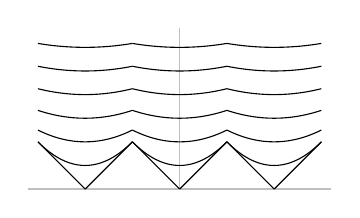
\begin{tikzpicture}[scale=1.2]
\draw [line width=0.2mm,lightgray] (-1.6,0)--(1.6,0);
\draw [line width=0.2mm,lightgray] (0, 0)--(0,1.7);
\draw[domain= -1.5:-1,smooth,variable=\x]  plot ({\x} , {-\x-1});
\draw[domain= -1:-0.5,smooth,variable=\x]  plot ({\x} , {\x+1});
\draw[domain= -0.5:0,smooth,variable=\x]  plot ({\x} , {-\x});
\draw[domain= 0:0.5,smooth,variable=\x]  plot ({\x} , {\x});
\draw[domain= 0.5:1,smooth,variable=\x]  plot ({\x} , {-\x+1});
\draw[domain= 1:1.5,smooth,variable=\x]  plot ({\x} , {\x-1});
\draw[domain=-1.5:-0.5,smooth,variable=\x ]  plot ({\x} , {(0.5^2+(\x+1)*(\x+1))/(2*1/2)});
\draw[domain=-0.5:0.5,smooth,variable=\x ]  plot ({\x} , {(0.5^2+\x*\x)/(2*1/2)});
\draw[domain=0.5:1.5,smooth,variable=\x ]  plot ({\x} , {(0.5^2+(\x-1)*(\x-1))/(2*1/2)});
\draw[domain=-1.5:-0.5,smooth,variable=\x ]  plot ({\x} , {(1^2+(\x+1)*(\x+1))/(2*1)});
\draw[domain=-0.5:0.5,smooth,variable=\x ]  plot ({\x} , {(1^2+\x*\x)/(2*1)});
\draw[domain=0.5:1.5,smooth,variable=\x ]  plot ({\x} , {(1^2+(\x-1)*(\x-1))/(2*1)});
\draw[domain=-1.5:-0.5,smooth,variable=\x ]  plot ({\x} , {(1.5^2+(\x+1)*(\x+1))/(2*1.5)});
\draw[domain=-0.5:0.5,smooth,variable=\x ]  plot ({\x} , {(1.5^2+\x*\x)/(2*1.5)});
\draw[domain=0.5:1.5,smooth,variable=\x ]  plot ({\x} , {(1.5^2+(\x-1)*(\x-1))/(2*1.5)});
\draw[domain=-1.5:-0.5,smooth,variable=\x ]  plot ({\x} , {(2^2+(\x+1)*(\x+1))/(2*2)});
\draw[domain=-0.5:0.5,smooth,variable=\x ]  plot ({\x} , {(2^2+\x*\x)/(2*2)});
\draw[domain=0.5:1.5,smooth,variable=\x ]  plot ({\x} , {(2^2+(\x-1)*(\x-1))/(2*2)});
\draw[domain=-1.5:-0.5,smooth,variable=\x ]  plot ({\x} , {(2.5^2+(\x+1)*(\x+1))/(2*2.5)});
\draw[domain=-0.5:0.5,smooth,variable=\x ]  plot ({\x} , {(2.5^2+\x*\x)/(2*2.5)});
\draw[domain=0.5:1.5,smooth,variable=\x ]  plot ({\x} , {(2.5^2+(\x-1)*(\x-1))/(2*2.5)});
\draw[domain=-1.5:-0.5,smooth,variable=\x ]  plot ({\x} , {(3^2+(\x+1)*(\x+1))/(2*3)});
\draw[domain=-0.5:0.5,smooth,variable=\x ]  plot ({\x} , {(3^2+\x*\x)/(2*3)});
\draw[domain=0.5:1.5,smooth,variable=\x ]  plot ({\x} , {(3^2+(\x-1)*(\x-1))/(2*3)});
\end{tikzpicture}
\caption{Hydrodynamic limits of periodic height function when $t=O(t)$}
\label{fig:Ringmaro}
	\end{minipage}
\end{figure}


The number $N$ of particles in the TASEP on the ring is preserved. 
%Let $N$ be an integer satisfying $1\le N\le L$, representing the number of particles. 
We assume the step initial condition shown in Figure \ref{fig:Ring}. 
For the convenience of presentation, we assume that $L$ is an even integer and $N=L/2$ so that the particle density $\rho=N/L=1/2$. 
The initial height function of the periodic TASEP is the bottom curve in Figure \ref{fig:Ringmaro}. 
The other curves are the hydrodynamic limits, as time $t$ and period $L$ tend to infinity proportionally when $t/L=0.5n$ for $n=1,2, \cdots, 6$. 

Consider two cases, one that $t\to\infty$ with $L$ fixed and the other that $L\to\infty$ with $t$ fixed. 
If $t\to\infty$ with $L$ fixed, the periodic corner growth model becomes essentially a one-dimensional growth model, and we expect that the height scales as $t^{1/2}$ and converges to the Gaussian distribution. 
On the other hand, if $L\to \infty$ with $t$ fixed, then the periodic TASEP becomes the usual TASEP on $\Z$. 
Thus, the height scales as $t^{1/3}$ if we let $t\to\infty$ after taking $L\to \infty$. 
An interesting intermediate regime is when $L, t\to\infty$ simultaneously such that 
\beq \label{eq:relax}
	t=O(L^{3/2}). 
\eeq
Since the spatial scale for KPZ limit theorems on infinite spaces is $t^{2/3}$, we expect that the height functions at all positions on the ring of size $L$ are correlated non-trivially. 
%we expect the positions of distance $O(L)$ to be critically correlated  in the regime \eqref{eq:relax}. In other words, the height functions at all positions on the ring are correlated non-trivially. 
%The limit distribution should depend on $\tau = t L^{-2/3}$. 
%The paper \cite{Baik-Liu16} showed that if $t\ll L^{3/2}$, then the one-point distribution converges to the same limit as the KPZ fixed points on infinite space. 
If \eqref{eq:relax} holds, we say that we are in the relaxation time regime. 


There were some results on transition probabilities and the spectral gap of the generator in the relaxation time regime, such  as \cite{Gwa-SpohnBethe}.  
However, KPZ limit theorems %in the relaxation time regime 
were obtained only recently. 
The paper \cite{Prolhac16}, which is a non-completely rigorous physics paper, and \cite{Baik-Liu18} obtained a one-point KPZ limit theorem almost at the same time independently. 
This result was further extended to 2d multi-point distributions in \cite{Baik-Liu19, Baik-Liu21}. 
%We state a result of \cite{Baik-Liu19}. 

\begin{theorem}[\cite{Baik-Liu19}] \label{thm:PTASEP}
Consider the TASEP on a ring of size $L$ with the step initial condition and extend it to the periodic TASEP. 
% and let $\pkheight$ be the associated periodic height function with $\pkheight(0,0)=0$. 
Assume that $L$ is even and $\rho=N/L= 1/2$ for the convenience of presentation. 
Set 
\beqq
	T=L^{3/2}. 
\eeqq
For $i=1, \cdots, m$, let 
%\beqq
%	\ptap_i =\pkga_i T^{2/3}, \qquad  \ptat_i = 2 \pkt_i T , \qquad	\ptah_i= \frac{\ptat_i}2  -  \pkh_i T^{1/3}
%\eeqq
 $(\pkga_i,  \pkt_i, \pkh_i) \in \R \times  \R_+\times \R$ and assume that $\pkt_1<\cdots< \pkt_m$. 
Then, %the periodic height function satisfies 
\beqq
	\lim_{T\to \infty} \Prob \Big( \bigcap_{i=1}^m  \big\{  \frac{\pkheight(\pkga_i T^{2/3}, 2 \pkt_i T) - \pkt_i T}{-T^{1/3}} \le \pkh_i   \big\} \Big) 
	=   \pkFdist_m(\pkh; \pkga, \pkt)
%	\lim_{T\to \infty} \Prob \Big( \bigcap_{i=1}^m  \{ \pkheight(\ptap_i, \ptat_i)\le \ptah_i \} \Big) 
%	=   \pkFdist_m(\pkh; \pkga, \pkt)
\eeqq
for an $m$-point distribution function $\pkFdist_m$ described in the next section. 
\end{theorem}

Like the infinite space case, we expect that the height field of the periodic models in the relaxation time regime converges to a universal field, which we may call the periodic KPZ fixed point. 
The function $\pkFdist_m$ should be the $m$-point distribution of this conjectured periodic KPZ fixed point with the (periodic) narrow wedge initial condition. 
It is naturally periodic with respect to $\pkga_i\mapsto \pkga_i+1$. 
However, unlike the KPZ fixed point, $\pkFdist_m$ is not invariant under the rescaling \eqref{eq:rescale}. 
Indeed, we conjecture that $\pkFdist_m$ interpolates the KPZ fixed point and one-dimensional Brownian motion. Concretely, we expect that  
\beqq
	 \lim_{\epsilon\to 0} \pkFdist_m(\pkh^\epsilon; \pkga^\epsilon, \pkt^\epsilon) =  \kFdist_m(\pkh; \pkga, \pkt) 
	 \qquad \text{where $(\pkh_i^\epsilon, \pkga_i^\epsilon, \pkt_i^\epsilon) = ( (\pkt_i \epsilon)^{1/3}\pkh_i, (\pkt_i \epsilon)^{2/3} \pkga_i,  \pkt_i \epsilon)$} 
\eeqq
and $\kFdist_m$ is the $m$-point distribution of the KPZ fixed point, and that 
\beqq
	\lim_{s\to \infty} \pkFdist_m ( \pkh^s; \pkga,  \pkt^s  )  = G_m(\pkh; \pkt) %\to \frac1{\sqrt{2\pi}} \int_{-\infty}^{\pkh_1} e^{-y^2/x} \dd y 
	\qquad \text{where $( \pkh_i^s, \pkt^s) = ( - s \pkt_i + \frac{s^{1/2} \pi^{1/4} }{\sqrt{2}} \pkh_i, s \pkt_i)$ }
\eeqq
and $G_m$ is the $m$-point distribution of a Brownian motion at times $\pkt_1, \cdots, \pkt_m$. 
These conjectures were proved for $m=1$ in \cite{Baik-Liu-Silva20}, assuming $\pkga_1=0$ for the $\epsilon\to 0$ case. 


%If we take $L\to \infty$ before taking $T\to \infty$, then we obtain the finite-time multi-point distribution of the TASEP on $\Z$. 
%This limit is tricky to take but was obtained by \cite{Liu19} from which Liu obtained his result on the multi-point distribution of the KPZ fixed point. 

%The result of \cite{Liu19} on the multi-point distributions of the TASEP on the infinite space was actually derived from the result of \cite{Baik-Liu19} on the periodic domain and then taking the large period from it. 
%Algebraically it appears that the periodic domain is easier to compute the multi-point, especially multi-time, distributions. 
%We state a result from \cite{Baik-Liu19}. 

Theorem \ref{thm:PTASEP} is also proved for the discrete-time TASEP on a ring \cite{Liao21}. 
However,  extending the result to other integrable models is at the moment a challenge. 


%%%%%%%%%%%%%%%%%%%%%%%%%%%%%%%%%%%%%%%%%%%%%%%%%%%%%%%%%%%%%
\section{Formula of multi-point distribution functions} \label{sec:dfformula}

%%%%%%%%%%%%%%%%%%%%%%%%%%%%%%%%%%%%%%%%%%%%%%%%%%%%%%%%%%%%%
\subsection{Formula for KPZ fixed point}

Let $\kFdist_m$ be the $m$-point distribution of the KPZ fixed point with the narrow wedge initial condition. The result of  \cite{Liu19} implies that  
\beq \label{eq:KPZformula}
	\kFdist_m(\kh; \kga, \kt) 
	= \frac1{(2\pi \ii)^{m-1}} \oint \cdots \oint  \frac{\det( \kid- \kK_\zeta)}{\zeta_1(1-\zeta_1) \cdots \zeta_{m-1} (1-\zeta_{m-1})} \dd \zeta_1 \cdots \dd \zeta_{m-1}
\eeq
where $\zeta=(\zeta_1, \cdots, \zeta_{m-1})$, and the contours are nested circles of radii less than $1$ centered at the origin. 
The operator $\kK_\zeta$ acts on $L^2(\Sigma)$, where 
$\Sigma$ is the union of $4m-2$ contours in Figure \ref{fig:KPZcontour} that extend to infinity with angle $\pi/5$ from the $x$-axis.
The kernel of $\kK_\zeta$ can be written \cite{Baik-Prokhorov-Silva21}  as a simple conjugation of the kernel 
\beq \label{eq:kpzKkernel}
	\kK^{\mathrm{conj}}_\zeta(\ku, \kv) = \frac{\ka(\ku)^T \kD(\ku)^T \kD(\kv) \kb( \kv)}{\ku-\kv}, \qquad \ku, \kv\in \Sigma, 
\eeq
which is zero for $\ku=\kv$. 
The $(m+1)\times (m+1)$ matrix 
\beqq
	\kD(z)= \diag\big( e^{- \frac{1}{3} \kt_1 z^3+ \frac{1}{2} \kga_1 z^2 + \kh_1 z}, \cdots, e^{- \frac{1}{3} \kt_m z^3 + \frac{1}{2} \kga_m z^2 + \kh_m z}, 1 \big) . 
\eeqq
The $(m+1)\times 1$ vectors $\ka(z)$ and $\kb(z)$ are simple and explicit, and they do not depend on $\kh_i, \kga_i, \kt_i$. 
%We only note that $\hat\ka(z)$ and $\hat\kb(z)$ depend on $\zeta_i$, but they do not depend on $\kt_i, \kga_i, \kh_i$, but depend on $\zeta_i$. 
Note that the exponent $- \frac{1}{3} \kt_i z^3+ \frac{1}{2} \kga_i z^2+ \kh_i z$ in $\kD(z)$ is unchanged if we rescale as \eqref{eq:rescale} and $z\mapsto \alpha^{-1} z$. 
This is consistent with the rescaling property of the KPZ fixed point. 

\begin{figure}
\centering
\begin{minipage}{.4\textwidth}\centering
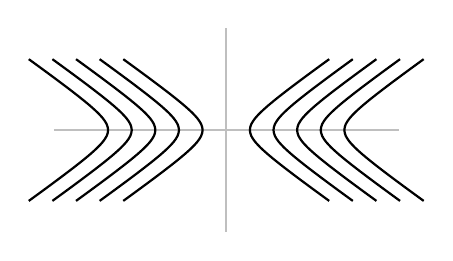
\begin{tikzpicture}[scale=0.3]
\draw [line width=0.2mm,lightgray] (-7.3,0)--(7.3,0);
\draw [line width=0.2mm,lightgray] (0,-4.3)--(0,4.3);
\draw[domain=-3:3,smooth,variable=\y, thick]  plot ({-(2*\y*\y+1)^(1/2)},{\y});
\draw[domain=-3:3,smooth,variable=\y, thick]  plot ({-1-(2*\y*\y+1)^(1/2)},{\y});
\draw[domain=-3:3,smooth,variable=\y, thick]  plot ({-2-(2*\y*\y+1)^(1/2)},{\y});
\draw[domain=-3:3,smooth,variable=\y, thick]  plot ({-3-(2*\y*\y+1)^(1/2)},{\y});
\draw[domain=-3:3,smooth,variable=\y, thick]  plot ({-4-(2*\y*\y+1)^(1/2)},{\y});
\draw[domain=-3:3,smooth,variable=\y, thick]   plot ({(2*\y*\y+1)^(1/2)},{\y});
\draw[domain=-3:3,smooth,variable=\y, thick]  plot ({1+(2*\y*\y+1)^(1/2)},{\y});
\draw[domain=-3:3,smooth,variable=\y, thick]   plot ({2+(2*\y*\y+1)^(1/2)},{\y});
\draw[domain=-3:3,smooth,variable=\y, thick]  plot ({3+(2*\y*\y+1)^(1/2)},{\y});
\draw[domain=-3:3,smooth,variable=\y, thick]   plot ({4+(2*\y*\y+1)^(1/2)},{\y});
\end{tikzpicture}
\caption{The space $\Sigma$ for KPZ fixed point when $m=3$}
\label{fig:KPZcontour}
\end{minipage}
\quad
\begin{minipage}{.45\textwidth}\centering
%\hspace{1cm}
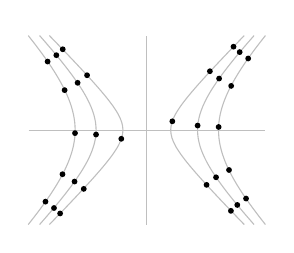
\begin{tikzpicture}[scale=0.3]
\draw [lightgray] (-5,0)--(5,0);
\draw [lightgray] (0,-4)--(0,4);
\draw[domain=-4:4,smooth,variable=\y,lightgray]  plot ({-(\y*\y+1.02)^(1/2)},{\y});   %x^2-y^2=-2\ln(0.6)
\draw[domain=-4:4,smooth,variable=\y,lightgray]  plot ({-(\y*\y+4.61)^(1/2)},{\y});   %x^2-y^2=-2\ln(0.1)
\draw[domain=-4:4,smooth,variable=\y,lightgray]  plot ({-(\y*\y+9.21)^(1/2)},{\y});   %x^2-y^2=-2\ln(0.01)
\draw[domain=-4:4,smooth,variable=\y,lightgray]  plot ({(\y*\y+1.02)^(1/2)},{\y});   %x^2-y^2=-2\ln(0.6)
\draw[domain=-4:4,smooth,variable=\y,lightgray]  plot ({(\y*\y+4.61)^(1/2)},{\y});   %x^2-y^2=-2\ln(0.1)
\draw[domain=-4:4,smooth,variable=\y,lightgray]  plot ({(\y*\y+9.21)^(1/2)},{\y});   %x^2-y^2=-2\ln(0.01)
\fill (-3.93, -3.30) circle[radius=3.5pt] node [above,shift={(0pt,0pt)}] {};   %z=(0.1)e^{-0.4 i}
\fill (-3.06, -2.18) circle[radius=3.5pt] node [above,shift={(0pt,0pt)}] {};
\fill (-2.15, -0.19) circle[radius=3.5pt] node [above,shift={(0pt,0pt)}] {};
\fill (-2.93, 2.00) circle[radius=3.5pt] node [above,shift={(0pt,0pt)}] {};
\fill (-3.83, 3.17) circle[radius=3.5pt] node [above,shift={(0pt,0pt)}] {};
\fill (-3.67, -3.53) circle[radius=3.5pt] node [above,shift={(0pt,0pt)}] {};   %z=(0.6)e^{-0.4 i}
\fill (-2.67, -2.49) circle[radius=3.5pt] node [above,shift={(0pt,0pt)}] {};
\fill (-1.08, -0.37) circle[radius=3.5pt] node [above,shift={(0pt,0pt)}] {};
\fill (-2.53, 2.32) circle[radius=3.5pt] node [above,shift={(0pt,0pt)}] {};
\fill  (-3.56, 3.42) circle[radius=3.5pt] node [above,shift={(0pt,0pt)}] {};
\fill (-4.29, -3.03) circle[radius=3.5pt] node [above,shift={(0pt,0pt)}] {};    %z=(0.01)e^{-0.4 i}
\fill (-3.57, -1.87) circle[radius=3.5pt] node [above,shift={(0pt,0pt)}] {};
\fill (-3.04, -0.13) circle[radius=3.5pt] node [above,shift={(0pt,0pt)}] {};
\fill (-3.48, 1.69) circle[radius=3.5pt] node [above,shift={(0pt,0pt)}] {};
\fill  (-4.20, 2.90) circle[radius=3.5pt] node [above,shift={(0pt,0pt)}] {};
\fill (3.93, 3.30) circle[radius=3.5pt] node [above,shift={(0pt,0pt)}] {};   %z=(0.1)e^{-0.4 i}
\fill (3.06, 2.18) circle[radius=3.5pt] node [above,shift={(0pt,0pt)}] {};
\fill (2.15, 0.19) circle[radius=3.5pt] node [above,shift={(0pt,0pt)}] {};
\fill (2.93, -2.00) circle[radius=3.5pt] node [above,shift={(0pt,0pt)}] {};
\fill (3.83, -3.17) circle[radius=3.5pt] node [above,shift={(0pt,0pt)}] {};
\fill (3.67, 3.53) circle[radius=3.5pt] node [above,shift={(0pt,0pt)}] {};   %z=(0.6)e^{-0.4 i}
\fill (2.67, 2.49) circle[radius=3.5pt] node [above,shift={(0pt,0pt)}] {};
\fill (1.08, 0.37) circle[radius=3.5pt] node [above,shift={(0pt,0pt)}] {};
\fill (2.53, -2.32) circle[radius=3.5pt] node [above,shift={(0pt,0pt)}] {};
\fill  (3.56, -3.42) circle[radius=3.5pt] node [above,shift={(0pt,0pt)}] {};
\fill (4.29, 3.03) circle[radius=3.5pt] node [above,shift={(0pt,0pt)}] {};    %z=(0.01)e^{-0.4 i}
\fill (3.57, 1.87) circle[radius=3.5pt] node [above,shift={(0pt,0pt)}] {};
\fill (3.04, 0.13) circle[radius=3.5pt] node [above,shift={(0pt,0pt)}] {};
\fill (3.48, -1.69) circle[radius=3.5pt] node [above,shift={(0pt,0pt)}] {};
\fill  (4.20, -2.90) circle[radius=3.5pt] node [above,shift={(0pt,0pt)}] {};
\end{tikzpicture}
\caption{The space $\pspace$ for periodic KPZ fixed when $m=3$.}
\label{fig:periodicKPZset}
\end{minipage}
\end{figure}

%%%%%%%%%%%%%%%%%%%%%%%%%%%%%%%%%%%%%%%%%%%%%%%%%%%%%%%%%%%%%
\subsection{Periodic case}

The formula of \cite{Baik-Liu19} is 
\beq \label{eq:PKPZformula}
	\pkFdist_m(\pkh; \pkga, \pkt)
	= \oint \cdots \oint  \pkCdisc(\zeta) \det(\pid-\pK_\zeta)   \dd \zeta_1 \cdots \dd \zeta_{m}, 
\eeq
where this time there are $m$ integrals and $\pkCdisc(\zeta)$ is an explicit function expressed in terms of polylog functions. 
The kernel of the operator $\pK_\zeta$ is of the same form as \eqref{eq:kpzKkernel} but $\ka(z)$ and $\kb(z)$ are slightly different. 
The key change is the space for $\pK_{\zeta}$. It is $\ell^2(\pspace)$, where
$\pspace= \pspace_1\cup\cdots \cup \pspace_m$ and $\pspace_i$ is the discrete set of the roots of the equation 
\beq \label{eq:Betheeqlimit}
	e^{-s^2/2}= \zeta_i , 
\eeq
shown in Figure \ref{fig:periodicKPZset}. 
See the following subsection for how this equation arises. 


%%%%%%%%%%%%%%%%%%%%%%%%%%%%%%%%%%%%%%%%%%%%%%%%%%%%%%%%%%%%%
\subsection{Transition probabilities} \label{sec:Bethe}


We mentioned in Subsection \ref{sec:integrablemethod} that one way of proving a KPZ limit theorem for the TASEP is to compute the transition probabilities explicitly and then take an appropriate sum to find the finite-time distribution functions. 
The summation part is often more technical, but here we discuss the transition probabilities to see how \eqref{eq:Betheeqlimit} arises. 
 
Suppose that there are only $N$ particles for the TASEP on $\Z$. 
Let $\mathcal{W}_N= \{ (a_1, \cdots, a_N)\in \Z^N: a_1<\cdots< a_N\}$ be the ordered set of the particle locations. 
Sch\"utz \cite{Schutz97} showed that 
\beq \label{eq:tranpro}
	\Prob_{Y}(X; t) =  \det \left[ \frac1{2\pi \ii} \oint s^{j-i+1}(s+1)^{-x_i+y_j+i-j} e^{ts} \dd s \right]_{i,j=1}^N 
\eeq
for $X$ and $Y$ in $\mathcal{W}_N$, where the contour is a circle that encloses the points $s=0,-1$. 

For the periodic TASEP, the particle locations can be represented by the set 
\beqq
	\mathcal{W}_N^L=  \{ (a_1, \cdots, a_N)\in \Z^N: a_1<\cdots< a_N <a_1+L\} . 
\eeqq
Note that if we consider the TASEP on a ring, this set keeps track of global circulations of the particles. 
%Note that if we consider the TASEP on a ring, this set keeps track of how many rotations the particles make. 
We showed in \cite{Baik-Liu18} that 
\beq \label{eq:transprofper}
	\Prob_{Y}(X; t) = \oint \det \left[ \frac1{L} \sum_{w} \frac{w^{j-i+1}(w+1)^{-x_i+y_j+i-j} e^{tw}}{w+N/L} \right]_{i,j=1}^N  \frac{\dd z}{2\pi \ii z}
\eeq
for $X, Y\in \mathcal{W}_N^L$, where the integral contour for $z$ is any circle enclosing the origin, and the sum inside is over the roots of the equation 
\beq \label{eq:Betheequation}
	w^N (w+1)^{L-N}=z . 
\eeq 
See Figure \ref{fig:Betheroots}. 

\begin{figure}
\centering
\begin{minipage}{.25\textwidth}
\centering
\includegraphics[width=3cm]{Roots1b.pdf}
\end{minipage}
\begin{minipage}{.25\textwidth}
\centering
\includegraphics[width=3cm]{Roots2b.pdf}
\end{minipage}
\begin{minipage}{.25\textwidth}
\centering
\includegraphics[width=3cm]{Roots3b.pdf}
\end{minipage}
\caption{Bethe roots when $L=24$ and $N=8$ for three values of $z$}
\label{fig:Betheroots}
\end{figure}

We now explain the equation \eqref{eq:Betheequation}. 
Due to the periodicity, if $A=(a_1, \cdots, a_N)$ is in $\mathcal{W}_N(L)$, then $A'=(a_2, \cdots, a_N, a_1+L)$ also represents the same particle configuration of the periodic TASEP. 
Thus, the transition probability should remain the same if we replace $(x_1, \cdots, x_N)$ and $(y_1, \cdots, y_N)$ by $(x_2, \cdots, x_N, x_1+L)$ and $(y_2, \cdots, y_N, y_1+L)$, respectively. 
We can check directly that the determinant in \eqref{eq:transprofper} is unchanged thanks to the equation \eqref{eq:Betheequation}. 
Equation \eqref{eq:Betheequation} takes care of the labeling ambiguity in the periodic case. 
Here the variable $z$ could have been any fixed constant, but making it as a free parameter turns out to be the right choice. 
Since \eqref{eq:tranpro} and \eqref{eq:transprofper} were found by solving the Kolmogorov forward equation using the Bethe ansatz method, the roots of \eqref{eq:Betheequation} are called the Bethe roots. 

Now, if we set $L=2N$, $w= -\frac12 + \frac{s}{2\sqrt{2N}}$, and $z= (-4)^{-N} \zeta$ in \eqref{eq:Betheequation}, and let $N\to \infty$, then the equation becomes $e^{-s^2/2}=\zeta$, which is \eqref{eq:Betheeqlimit}. 


 


%These results were obtained finding the transition probabilities and summing them up. 
%A Schur measure-like structure is still missing as well as extensions to other models. 


%%%%%%%%%%%%%%%%%%%%%%%%%%%%%%%%%%%%%%%%%%%%%%%%%%%%%%%%%%%%%
\section{Integrable differential equations} \label{sec:integrableDE}

Distribution functions of the KPZ fixed point have connections to deterministic integrable differential equations. 
As proved in 1994 \cite{Tracy-Widom94}, the Tracy-Widom distribution is expressible in terms of the Painlev\'e II equation, one of a family of six special nonlinear ordinary differential equations  \cite{Fokas-Its-Kitaev-Novokshenov06}. 
The papers \cite{Tracy-Widom03, Adler-van_Moerbeke05, Wang08a, Bertola-Cafasso-2012b, Quastel-Remenik19b} also found differential equations for equal-time, multi-position distribution functions of the KPZ fixed point. 
We state the following result for multi-point distributions for both infinite and periodic domains. % with step initial conditions. 

%the work  \cite{Tracy-Widom94} of Tracy and Widom in 1994 that expresses the Tracy-Widom distribution in terms of the Painlev\'e II equation, one of six special nonlinear ordinary differential equations  \cite{Fokas-Its-Kitaev-Novokshenov06}. 

Define the parameters
\beqq
	\knt_i= \kt_i/3, %\frac{-\kt}{3}, 
	\qquad \kny_i=\kga_i, %\frac{\kga}{2}, 
	\qquad \knx_i= \kh_i, 
\eeqq
and let
\beqq
	\partial_{\knt}= \sum_{i=1}^m \partial_{\knt_i}, \qquad
	\partial_{\kny}= \sum_{i=1}^m \partial_{\kny_i}, \qquad
	\partial_{\knx}= \sum_{i=1}^m \partial_{\knx_i}. 
\eeqq

\begin{theorem}[\cite{Baik-Liu-Silva20, Baik-Prokhorov-Silva21}] \label{thm:mKdV}
Let $\kK=\kK_\zeta$ be the operator in either \eqref{eq:KPZformula} or \eqref{eq:PKPZformula}. 
If $\det(\kid- \kK)\neq 0$, which holds for all but at most countably many parameters, then 
\beqq
	\partial^2_{\knx} \log \det(\kid- \kK) = - \kr^T\kp
\eeqq
for complex-valued $m\times 1$ vector functions $\kp(\knt, \kny, \knx)$ and $\kr(\knt, \kny, \knx)$ which satisfy the equations
\beq \label{eq:NLS}
	\partial_{\kny} \kp = \frac12 \partial_{\knx}^2 \kp -  \kp \kr^T \kp, \qquad
	\partial_{\kny} \kr = -\frac12 \partial_{\knx}^2 \kr +  \kr \kp^T \kr
\eeq
and  
\beq \label{eq:mKdV}
	\partial_{\knt} \kp + \partial_{\knx}^3 \kp - 3 (\partial_{\knx} \kp) \kr^T \kp  - 3 \kp \kr^T (\partial_{\knx} \kp) =0 , \quad
	\partial_{\knt} \kr + \partial_{\knx}^3 \kr - 3  (\partial_{\knx} \kr) \kp^T \kr -  3 \kr \kp^T (\partial_{\knx} \kr ) =0. 
\eeq
\end{theorem}

Equation \eqref{eq:mKdV} is a coupled system of vector-valued modified Korteweg-De Vries (mKdV) equations. 
The scalar mKdV equation is 
$\partial_{\knt} f + \partial_{\knx}^3 f - 6 (\partial_{\knx} f) f^2  =0$. 
On the other hand,  equation \eqref{eq:NLS} forms a coupled system of vector-valued nonlinear forward and backward heat equations. 
They become vector-valued nonlinear Sch{\"o}dinger (NLS) equations if we change $\kny_i\mapsto \ii \kny_i$. 
NLS and mKdV equations are two of the most famous integrable partial differential equations \cite{Ablowitz-Clarkson91}. 
The above two systems of equations can be combined to the Kadomtsev-Petviashvili (KP) equation, another integrable differential equation in three variables.
%Here $\kp$ and $\kr$ are unusual solutions since they are complex-valued. 
Theorem \ref{thm:mKdV} was obtained using the fact that the operator is a so-called integrable operator \cite{IIKS, Deift99b}. 
%Integrable operators are connected to Riemann--Hilbert problems \cite{IIKS, Deift99b}. See also \cite{Bothner21}. 


Integrable differential equations have a long history starting with the work of Gardner, Greene, Kruskal, and Miura in 1967. 
They found a scattering transform method, an equation-specific nonlinear Fourier transform, to solve the Korteweg-De Vries equation.  
Like the integrable models in the KPZ universality class, integrable differentiable equations are isolated examples of nonlinear differential equations that can often be solved explicitly and analyzed asymptotically. See, for example, \cite{Ablowitz-Clarkson91, Deift19}. 
It is intriguing that integrable probability models are related to integrable differential equations. 


%The recent paper \cite{Matetski-Quastel-Remenik17} introduced the Brownian scattering method, which maps an initial condition for the KPZ fixed point to an operator, and showed that the evolution by the KPZ fixed point implies a linearization of the evolution of the operator, and the Fredholm determinant is an inverse transform that gives the equal-time distribution. 
%It is desired to see further progress here. 



%%%%%%%%%%%%%%%%%%%%%%%%%%%%%%%%%%%%%%%%%%%%%%%%%%%%%%%%%%%%%
\section{Comments on universality} \label{sec:univ}

%We complete this article with some comments on universality. 
KPZ limit theorems are proved for many isolated examples of integrable models. %, but these are still isolated examples. 
%The KPZ universality question is still a challenge. 
In this final section, we discuss a few instances that universality is proved. 


%%%%%%%%%%%%%%%%%%%%%%%%%%%%%%%%%%%%%%%%%%%%%%%%%%%%%%%%%%%%%
\subsection{Thin DLPP}


The universality should hold for the last passage time $L(n,k)$ as $n,k\to \infty$.
It is easy to prove it for thin rectangles. 
Recall from Subsection \ref{sec:DLPP} that $w_s$ denotes the random variable at site $s\in \Z$, representing the passage time through the site. 

\begin{theorem}[\cite{Baik-Suidan05, Bodineau-Martin05}]  \label{thm:thin}
Suppose that $w_s$ is an arbitrary random variable which has all moments. Assume that the mean is zero and the variance is one. Then, for every $x$, 
\beqq
	\lim_{n, k \to \infty} \Prob\Big( \frac{L(n, k )- 2 \sqrt{nk}}{n^{\frac12} k^{-\frac16}} \le x \Big) = \FTW(x) \quad \text{for $k=[n^a]$}
\eeqq
with any $0<a<3/7$. 
\end{theorem}

The restriction $a<3/7$ is technical. If we assume only finite $p$ moments for $p>2$, then the result holds for thinner rectangles satisfying $0<a<\frac{3(p-2)}{7 p}$. 

\begin{figure}
\centering
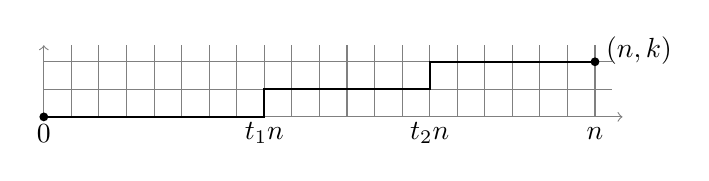
\begin{tikzpicture}[scale=0.7]
\draw [->, thin][gray] (0,0) to (10.5,0);
\draw [->, thin][gray] (0,0) to (0, 1.3);
\draw [-, thin, gray] (0,0.5) to (10.3,0.5);
\draw [-, thin, gray] (0,1) to (10.3,1);
\draw [-, thin, gray] (0.5,0) to (0.5,1.3);
\draw [-, thin, gray] (1,0) to (1,1.3);
\draw [-, thin, gray] (1.5,0) to (1.5,1.3);
\draw [-, thin, gray] (2,0) to (2,1.3);
\draw [-, thin, gray] (2.5,0) to (2.5,1.3);
\draw [-, thin, gray] (3,0) to (3,1.3);
\draw [-, thin, gray] (3.5,0) to (3.5,1.3);
\draw [-, thin, gray] (4,0) to (4,1.3);
\draw [-, thin, gray] (4.5,0) to (4.5,1.3);
\draw [-, thin, gray] (5,0) to (5,1.3);
\draw [-, thin, gray] (5.5,0) to (5.5,1.3);
\draw [-, thin, gray] (6,0) to (6,1.3);
\draw [-, thin, gray] (6.5,0) to (6.5,1.3);
\draw [-, thin, gray] (7,0) to (7,1.3);
\draw [-, thin, gray] (7.5,0) to (7.5,1.3);
\draw [-, thin, gray] (8,0) to (8,1.3);
\draw [-, thin, gray] (8.5,0) to (8.5,1.3);
\draw [-, thin, gray] (9,0) to (9,1.3);
\draw [-, thin, gray] (9.5,0) to (9.5,1.3);
\draw [-, thin, gray] (10,0) to (10,1.3);
\draw [-, thick] (0,0) to (4,0) to (4,0.5) to (7, 0.5) to (7, 1) to (10,1);
\fill (0,0) circle(0.08);
\fill (10,1) circle(0.08);
\node at (10.8, 1.2)  {$(n,k)$};
\node at (0, -0.3)  {$0$};
\node at (4, -0.3)  {$t_1n$};
\node at (7, -0.3)  {$t_2n$};
\node at (10, -0.3)  {$n$};
\end{tikzpicture}
\caption{Thin DLPP}
\label{fig:thin}
\end{figure}


For the case of fixed $k$ and large $n$, a directed path looks like the one in Figure \ref{fig:thin}. Since the sum of $w_s$ on each row converges to a Brownian motion, Donsker's theorem implies that 
\beqq
	 \frac{L(n,k)}{\sqrt{n}} \Rightarrow   D_k \quad \text{where $D_k= \sup_{0=t_0\le t_1\le \cdots\le t_k=1} \sum_{i=1}^k (B_i(t_i)- B_i(t_{i-1}))$}
\eeqq
and $B_i(t)$, $i=1, \cdots, k$, are independent Brownian motions. 
%This holds for general $w(p)$ with two finite moments. 
On the other hand, it is known \cite{Baryshnikov01} that  
\beqq
	\lim_{k\to \infty} \Prob( (D_k- 2\sqrt{k})k^{1/6} \le x) = \FTW(x). 
\eeqq
This limit is a consequence of an explicit formula of the exponential DLPP by letting $n\to\infty$ first and then taking $k\to \infty$. 
%This limit holds because $D_k$ is distributed as the largest eigenvalue of the Gaussian Hermitian random matrix: see Subsection \ref{sec:TASEPRM} below. 
We prove Theorem \ref{thm:thin} by showing that if $n, k\to \infty$ but $k$ grows slowly enough, we can take $n\to \infty$ first and $k\to \infty$ later. 
This argument is achieved by the Skorohod embedding or the Koml\'os--Major--Tusn\'ady embedding. 
However, the proof breaks down if $\alpha\ge 3/7$ since we cannot ignore the upward parts of the paths anymore. 
For $k=O(n)$, limit theorems are proved only for a few examples. % of random variables $w_s$ and a few variations of the models.  
 

%%%%%%%%%%%%%%%%%%%%%%%%%%%%%%%%%%%%%%%%%%%%%%%%%%%%%%%%%%%%%
\subsection{Interacting particle systems}

The particles in the TASEP move only one site to the right. Consider a more general finite-range exclusion process in which a particle at site $0$ can potentially move to site $v$ at rate $p(v)$. 
Assume that $\{v: p(v)>0\}$ is a finite set  generating $\Z$ additively, and $\sum_v v p(v)\neq 0$. 
In a recent paper \cite{Quastel-Sakar20}, Quastel and Sakar proved a KPZ limit theorem for finite-range exclusion processes started from a certain class of initial conditions. 
They compared the transition probabilities of the general process with those of the TASEP using energy estimates. 
This work is the first universality result in the $k=O(n)$ regime. It is exciting to see how the method further generalizes.  

%%%%%%%%%%%%%%%%%%%%%%%%%%%%%%%%%%%%%%%%%%%%%%%%%%%%%%%%%%%%%
\subsection{TASEP, Coulomb gas, and random matrices} \label{sec:TASEPRM}


In proving Theorem \ref{thm:Johansson}, Johansson also proved an unexpected connection of TASEP to Coulomb gas and random matrices \cite{Johansson00}. 
Consider the probability density function on $\R_+^n$ given by 
\beq \label{eq:Coulomb}
	p(x_1, \cdots, x_n) = c_{n, m} e^{2\sum_{1\le i<j\le n} \log |x_j-x_i|- \sum_{i=1}^n V(x_i) }, 
	\quad V(x)= x-(m-n)\log x, 
\eeq
where $c_{m,n}$ is the normalization constant.  
Let $x_{\max}=\max\{x_1, \cdots, x_n\}$. 
%Using the relation of the TASEP and the Schur measure, 
Johansson proved that for $m\ge n$, the last passage time $L(m,n)$ of the exponential DLPP has the same distribution as $x_{\max}$. 
The density function \eqref{eq:Coulomb} is said to define a  Coulomb gas with potential $V$ on $\R_+$ since the term $\log |x_i-x_j|$ is the 2d Coulomb potential of two equal charges at $x_i$ and $x_j$. 
The function $V(x)$ represents the confining potential. 

Let $X$ be an $n\times m$ random matrix with entries that are independent complex normal variables of mean zero and variance $1/2$. 
The random matrix $W=XX^*$ is called the complex Wishart matrix, and its eigenvalue density function is precisely \eqref{eq:Coulomb} \cite{Forrester10}. 
Thus, $L(m,n)$ has the same distribution as the largest eigenvalue of a complex Wishart matrix. 
See also \cite{Borodin-Peche08}. 
The connection of the exponential DLPP to Coulomb gas and the random matrix is special, and we do not expect to hold for general random variables $w_s$. 

There are universality results for both Coulomb gas and random matrices. 
The Tracy-Widom limit theorem is proved for the Coulomb gases with a general potential $V$. 
The paper \cite{Deift-Kriecherbauer-McLaughlin-Venakides-Zhou99} showed the limit theorem for generic analytic potentials, and \cite{Baik-Kriecherbauer-McLaughlin-Miller07} proved for discrete Coulomb gases in which particles are restricted to be only on a discrete set. 

Universality is a central question in random matrix theory, and there have been remarkable successes. 
The largest eigenvalue of a large class of random Hermitian matrices with independent entries converges to the Tracy-Widom distribution  \cite{Soshnikov99, Tao-Vu10, Erdos-Knowles-Yau-Yin12, Lee-Yin14}. 


%%%%%%%%%%%%%%%%%%%%%%%%%%%%%%%%%%%%%%%%%%%%%%%%%%%%%%%%%%%%%
\subsection{Universality in many directions} \label{sec:univs}

We discussed that the TASEP with the step initial condition is connected to several areas: 
\begin{itemize}
\item interacting particle system
\item 1+1 random growth process
\item two-dimensional directed last passage percolation and directed polymer
\item Coulomb gas
\item random matrix
\end{itemize}
The TASEP also has interpretations as a random tiling model, and non-intersecting paths \cite{Johansson02, Gorin21}. 
We expect universality results to hold in all of these seven areas. 
The meaning of universality is  different in each area. For example, in random matrix theory, the largest eigenvalue of any random Hermitian matrix with independent and identically distributed entries with 4+$\epsilon$ finite moments converges to the same limit, the Tracy-Widom distribution. 
On the other hand, the 2d field limit of interacting particle systems depends on the initial condition, a special case of which has the Tracy-Widom distribution as its marginal. 
%It remains to develop a general theory that encompasses all of these areas and possibly more.  

Even though many universality results are proved for Coulomb gases and random matrices, it remains to establish similar results for other areas and develop a general theory that encompasses all of these areas and possibly more.  


%As a special case, the one-point distribution for the step initial condition is the Tracy-Widom distribution. 


%------
% Insert acknowledgments and information
% regarding funding at the end of the last
% section, i.e., right before the bibliography.
%------


\subsection*{Acknowledgements}


The author would like to thank Percy Deift, Zhipeng Liu, Andrei Prokhorov, and Guilherme Silva for helpful conversations. 
This work was partially supported by the NSF grant DMS-1954790.  


%------
% Insert the bibliography.
%------

\bibliographystyle{emss}
%\bibliography{bibliography}

%\begin{thebibliography}{99}


\def\cydot{\leavevmode\raise.4ex\hbox{.}}
\begin{thebibliography}{10}
\providecommand{\url}[1]{\texttt{#1}}
\providecommand{\urlprefix}{URL }
\providecommand{\eprint}[2][]{\url{#2}}

\bibitem{Ablowitz-Clarkson91}
M.~J. Ablowitz and P.~A. Clarkson, \emph{Solitons, nonlinear evolution
  equations and inverse scattering}. London Mathematical Society Lecture Note
  Series 149, Cambridge University Press, Cambridge, 1991.

\bibitem{Adler-van_Moerbeke05}
M.~Adler and P.~van Moerbeke, P{DE}s for the joint distributions of the
  {D}yson, {A}iry and sine processes. \emph{Ann. Probab.} \textbf{33} (2005),
  no.~4, 1326--1361.

\bibitem{Aldous-Diaconis99}
D.~Aldous and P.~Diaconis, Longest increasing subsequences: from patience
  sorting to the {B}aik-{D}eift-{J}ohansson theorem. \emph{Bull. Amer. Math.
  Soc. (N.S.)} \textbf{36} (1999), no.~4, 413--432.

\bibitem{Amir-Corwin-Quastel11}
G.~Amir, I.~Corwin, and J.~Quastel, Probability distribution of the free energy
  of the continuum directed random polymer in {$1+1$} dimensions. \emph{Comm.
  Pure Appl. Math.} \textbf{64} (2011), no.~4, 466--537.

\bibitem{Baik-Barraquand-Corwin-Suidan18}
J.~Baik, G.~Barraquand, I.~Corwin, and T.~Suidan, Pfaffian {S}chur processes
  and last passage percolation in a half-quadrant. \emph{Ann. Probab.}
  \textbf{46} (2018), no.~6, 3015--3089.

\bibitem{Baik-Deift-Johansson99}
J.~Baik, P.~Deift, and K.~Johansson, On the distribution of the length of the
  longest increasing subsequence of random permutations. \emph{J. Amer. Math.
  Soc.} \textbf{12} (1999), no.~4, 1119--1178.

\bibitem{Baik-Deift-Suidan}
J.~Baik, P.~Deift, and T.~Suidan, \emph{Combinatorics and random matrix
  theory}. Graduate Studies in Mathematics 172, American Mathematical Society,
  Providence, RI, 2016.

\bibitem{Baik-Kriecherbauer-McLaughlin-Miller07}
J.~Baik, T.~Kriecherbauer, K.~T.-R. McLaughlin, and P.~Miller, \emph{Discrete
  orthogonal polynomials}. Annals of Mathematics Studies 164, Princeton
  University Press, Princeton, NJ, 2007.

\bibitem{Baik-Liu18}
J.~Baik and Z.~Liu, Fluctuations of {TASEP} on a ring in relaxation time scale.
  \emph{Comm. Pure Appl. Math.} \textbf{71} (2018), no.~4, 747--813.

\bibitem{Baik-Liu19}
J.~Baik and Z.~Liu, Multipoint distribution of periodic {TASEP}. \emph{J. Amer.
  Math. Soc.} \textbf{32} (2019), no.~3, 609--674.

\bibitem{Baik-Liu21}
J.~Baik and Z.~Liu, Periodic {TASEP} with general initial conditions.
  \emph{Probab. Theory Related Fields} \textbf{179} (2021), no. 3-4,
  1047--1144.

\bibitem{Baik-Liu-Silva20}
J.~Baik, Z.~Liu, and G.~L.~F. Silva, Limiting one-point distribution of
  periodic {TASEP}. 
 \emph{Ann. Inst. Henri Poincar\'{e} Probab. Stat.} \textbf{58} (2022), no. 1,
  248--302. 

\bibitem{Baik-Prokhorov-Silva21}
J.~Baik, A.~Prokhorov, and G.~L.~F. Silva, Integrable structure of the
  multipoint distributions of {KPZ} fixed point. 2022, in preparation.

\bibitem{Baik-Rains01a}
J.~Baik and E.~M. Rains, The asymptotics of monotone subsequences of
  involutions. \emph{Duke Math. J.} \textbf{109} (2001), no.~2, 205--281.

\bibitem{Baik-Rains01}
J.~Baik and E.~M. Rains, Symmetrized random permutations. In \emph{Random
  matrix models and their applications}, pp. 1--19, Math. Sci. Res. Inst. Publ.
  40, Cambridge Univ. Press, Cambridge, 2001.

\bibitem{Baik-Suidan05}
J.~Baik and T.~M. Suidan, A {GUE} central limit theorem and universality of
  directed first and last passage site percolation. \emph{Int. Math. Res. Not.}
   (2005), no.~6, 325--337.

\bibitem{Barraquand-Borodin-Corwin-Wheeler18}
G.~Barraquand, A.~Borodin, I.~Corwin, and M.~Wheeler, Stochastic six-vertex
  model in a half-quadrant and half-line open asymmetric simple exclusion
  process. \emph{Duke Math. J.} \textbf{167} (2018), no.~13, 2457--2529.

\bibitem{Barraquand-Corwin16}
G.~Barraquand and I.~Corwin, The {$q$}-{H}ahn asymmetric exclusion process.
  \emph{Ann. Appl. Probab.} \textbf{26} (2016), no.~4, 2304--2356.

\bibitem{Baryshnikov01}
Y.~Baryshnikov, G{UE}s and queues. \emph{Probab. Theory Related Fields}
  \textbf{119} (2001), no.~2, 256--274.

\bibitem{Bertola-Cafasso-2012b}
M.~Bertola and M.~Cafasso, Riemann-{H}ilbert approach to multi-time processes:
  the {A}iry and the {P}earcey cases. \emph{Phys. D} \textbf{241} (2012), no.
  23-24, 2237--2245.

\bibitem{Bodineau-Martin05}
T.~Bodineau and J.~Martin, A universality property for last-passage percolation
  paths close to the axis. \emph{Electron. Comm. Probab.} \textbf{10} (2005),
  105--112.

\bibitem{Borodin-Corwin13}
A.~Borodin and I.~Corwin, Macdonald processes. \emph{Probab. Theory Related
  Fields} \textbf{158} (2014), no. 1-2, 225--400.

\bibitem{Borodin-Corwin-Ferrari14}
A.~Borodin, I.~Corwin, and P.~Ferrari, Free energy fluctuations for directed
  polymers in random media in {$1+1$} dimension. \emph{Comm. Pure Appl. Math.}
  \textbf{67} (2014), no.~7, 1129--1214.

\bibitem{Borodin-Corwin-Ferrari-Veto15}
A.~Borodin, I.~Corwin, P.~Ferrari, and B.~Vet\H{o}, Height fluctuations for the
  stationary {KPZ} equation. \emph{Math. Phys. Anal. Geom.} \textbf{18} (2015),
  no.~1, Art. 20, 95.

\bibitem{Borodin-Corwin-Gorin16}
A.~Borodin, I.~Corwin, and V.~Gorin, Stochastic six-vertex model. \emph{Duke
  Math. J.} \textbf{165} (2016), no.~3, 563--624.

\bibitem{Borodin-Corwin-Remenik13}
A.~Borodin, I.~Corwin, and D.~Remenik, Log-gamma polymer free energy
  fluctuations via a {F}redholm determinant identity. \emph{Comm. Math. Phys.}
  \textbf{324} (2013), no.~1, 215--232.

\bibitem{Borodin-Ferrari08}
A.~Borodin and P.~L. Ferrari, Large time asymptotics of growth models on
  space-like paths. {I}. {P}ush{ASEP}. \emph{Electron. J. Probab.} \textbf{13}
  (2008), no. 50, 1380--1418.

\bibitem{Borodin-Ferrari14}
A.~Borodin and P.~L. Ferrari, Anisotropic growth of random surfaces in {$2+1$}
  dimensions. \emph{Comm. Math. Phys.} \textbf{325} (2014), no.~2, 603--684.

\bibitem{Borodin-Ferrari-Prahofer-Sasamoto07}
A.~Borodin, P.~L. Ferrari, M.~Pr{\"a}hofer, and T.~Sasamoto, Fluctuation
  properties of the {TASEP} with periodic initial configuration. \emph{J. Stat.
  Phys.} \textbf{129} (2007), no. 5-6, 1055--1080.

\bibitem{Borodin-Ferrari-Sasamoto08}
A.~Borodin, P.~L. Ferrari, and T.~Sasamoto, Large time asymptotics of growth
  models on space-like paths. {II}. {PNG} and parallel {TASEP}. \emph{Comm.
  Math. Phys.} \textbf{283} (2008), no.~2, 417--449.

\bibitem{Borodin-Ferrari-Sasamoto08a}
A.~Borodin, P.~L. Ferrari, and T.~Sasamoto, Transition between {A}iry$_1$ and
  {A}iry$_2$ processes and {TASEP} fluctuations. \emph{Comm. Pure Appl. Math.}
  \textbf{61} (2008), no.~11, 1603--1629.

\bibitem{Borodin-Gorin16}
A.~Borodin and V.~Gorin, Lectures on integrable probability. In
  \emph{Probability and statistical physics in {S}t. {P}etersburg}, pp.
  155--214, Proc. Sympos. Pure Math. 91, Amer. Math. Soc., Providence, RI,
  2016.

\bibitem{Borodin-Peche08}
A.~Borodin and S.~P{\'e}ch{\'e}, Airy kernel with two sets of parameters in
  directed percolation and random matrix theory. \emph{J. Stat. Phys.}
  \textbf{132} (2008), no.~2, 275--290.

\bibitem{Corwin11}
I.~Corwin, The {K}ardar-{P}arisi-{Z}hang equation and universality class.
  \emph{Random Matrices Theory Appl.} \textbf{1} (2012), no.~1, 1130001, 76.

\bibitem{Corwin-Petrov16}
I.~Corwin and L.~Petrov, Stochastic higher spin vertex models on the line.
  \emph{Comm. Math. Phys.} \textbf{343} (2016), no.~2, 651--700.

\bibitem{Dauvergne-Ortmann-Virag18}
D.~Dauvergne, J.~Ortmann, and B.~Vir\'ag, The directed landscape. 2018,
  arXiv:1812.00309.

\bibitem{Deift99b}
P.~Deift, Integrable operators. In \emph{Differential operators and spectral
  theory}, pp. 69--84, Amer. Math. Soc. Transl. Ser. 2 189, Amer. Math. Soc.,
  Providence, RI, 1999.

\bibitem{Deift-Kriecherbauer-McLaughlin-Venakides-Zhou99}
P.~Deift, T.~Kriecherbauer, K.~T.-R. McLaughlin, S.~Venakides, and X.~Zhou,
  Uniform asymptotics for polynomials orthogonal with respect to varying
  exponential weights and applications to universality questions in random
  matrix theory. \emph{Comm. Pure Appl. Math.} \textbf{52} (1999), no.~11,
  1335--1425.

\bibitem{Deift19}
P.~A. Deift, Three lectures on "{F}ifty years of {K}d{V}: an integrable
  system". In \emph{Nonlinear dispersive partial differential equations and
  inverse scattering}, pp. 3--38, Fields Inst. Commun. 83, Springer, New York,
  [2019] \copyright 2019.

\bibitem{Dimitrov20}
E.~Dimitrov, Two-point convergence of the stochastic six-vertex model to the
  {A}iry process. 2020, arXiv:2006.15934.

\bibitem{Erdos-Knowles-Yau-Yin12}
L.~Erd{\H{o}}s, A.~Knowles, H.-T. Yau, and J.~Yin, Spectral statistics of
  {E}rd{\H{o}}s-{R}\'{e}nyi {G}raphs {II}: {E}igenvalue spacing and the extreme
  eigenvalues. \emph{Comm. Math. Phys.} \textbf{314} (2012), no.~3, 587--640.

\bibitem{Ferrari-Spohn16}
P.~L. Ferrari and H.~Spohn, On time correlations for {KPZ} growth in one
  dimension. \emph{SIGMA Symmetry Integrability Geom. Methods Appl.}
  \textbf{12} (2016), Paper No. 074, 23.

\bibitem{Fokas-Its-Kitaev-Novokshenov06}
A.~S. Fokas, A.~R. Its, A.~A. Kapaev, and V.~Y. Novokshenov, \emph{Painlev\'{e}
  transcendents}. Mathematical Surveys and Monographs 128, American
  Mathematical Society, Providence, RI, 2006.

\bibitem{Forrester10}
P.~J. Forrester, \emph{Log-gases and random matrices}. London Mathematical
  Society Monographs Series 34, Princeton University Press, Princeton, NJ,
  2010.

\bibitem{Forster-Nelson-Stephen77}
D.~Forster, D.~R. Nelson, and M.~J. Stephen, Large-distance and long-time
  properties of a randomly stirred fluid. \emph{Phys. Rev. A} \textbf{16}
  (1977), 732--749.

\bibitem{Gaudin14}
M.~Gaudin, \emph{The {B}ethe wavefunction}. Cambridge University Press, New
  York, 2014.

\bibitem{Gorin21}
V.~Gorin, \emph{Lectures on random lozenge tilings}. Cambridge Studies in
  Advanced Mathematics 193, Cambridge University Press, Cambridge, 2021.

\bibitem{Gwa-SpohnBethe}
L.-H. Gwa and H.~Spohn, Bethe solution for the dynamical-scaling exponent of
  the noisy burgers equation. \emph{Phys. Rev. A} \textbf{46} (1992), 844--854.

\bibitem{Hammersley72}
J.~M. Hammersley, A few seedlings of research. In \emph{Proceedings of the
  {S}ixth {B}erkeley {S}ymposium on {M}athematical {S}tatistics and
  {P}robability ({U}niv. {C}alifornia, {B}erkeley, {C}alif., 1970/1971), {V}ol.
  {I}: {T}heory of statistics}, pp. 345--394, 1972.

\bibitem{Huse-Henley85}
D.~A. Huse and C.~L. Henley, Pinning and roughening of domain walls in ising
  systems due to random impurities. \emph{Phys. Rev. Lett.} \textbf{54} (1985),
  2708--2711.

\bibitem{IIKS}
A.~R. Its, A.~G. Izergin, V.~E. Korepin, and N.~A. Slavnov, Differential
  equations for quantum correlation functions. In \emph{Proceedings of the
  {C}onference on {Y}ang-{B}axter {E}quations, {C}onformal {I}nvariance and
  {I}ntegrability in {S}tatistical {M}echanics and {F}ield {T}heory}, pp.
  1003--1037, 4, 1990.

\bibitem{Imamura-Mucciconi-Sasamoto22}
T.~Imamura, M.~Mucciconi, and T.~Sasamoto, Solvable models in the {KPZ} class: approach through periodic and free boundary {S}chur measures. 2022, arXiv:2204.08420.
  
\bibitem{Johansson00}
K.~Johansson, Shape fluctuations and random matrices. \emph{Comm. Math. Phys.}
  \textbf{209} (2000), no.~2, 437--476.

\bibitem{Johansson02}
K.~Johansson, Non-intersecting paths, random tilings and random matrices.
  \emph{Probab. Theory Related Fields} \textbf{123} (2002), no.~2, 225--280.

\bibitem{Johansson03}
K.~Johansson, Discrete polynuclear growth and determinantal processes.
  \emph{Comm. Math. Phys.} \textbf{242} (2003), no. 1-2, 277--329.

\bibitem{Johansson17}
K.~Johansson, Two time distribution in {B}rownian directed percolation.
  \emph{Comm. Math. Phys.} \textbf{351} (2017), no.~2, 441--492.

\bibitem{Johansson19}
K.~Johansson, The two-time distribution in geometric last-passage percolation.
  \emph{Probab. Theory Related Fields} \textbf{175} (2019), no. 3-4, 849--895.

\bibitem{Johansson-Rahman19}
K.~Johansson and M.~Rahman, Multitime distribution in discrete polynuclear
  growth. 
  \emph{Comm. Pure Appl. Math.} \textbf{74} (2021), no.~12, 2561--2627.



\bibitem{Kardar-Parisi-Zhang86}
M.~Kardar, G.~Parisi, and Y.-C. Zhang, Dynamic scaling of growing interfaces.
  \emph{Phys. Rev. Lett.} \textbf{56} (1986), 889--892.

\bibitem{Lee-Yin14}
J.~O. Lee and J.~Yin, A necessary and sufficient condition for edge
  universality of {W}igner matrices. \emph{Duke Math. J.} \textbf{163} (2014),
  no.~1, 117--173.

\bibitem{Liao21}
Y.~Liao, Multi-point distribution of discrete time periodic {TASEP}. \emph{Probab. Theory Related Fields} \textbf{182} (2022), no. 3-4, 1053--1131.


\bibitem{Liggett85}
T.~M. Liggett, \emph{Interacting particle systems}. Grundlehren der
  Mathematischen Wissenschaften [Fundamental Principles of Mathematical
  Sciences] 276, Springer-Verlag, New York, 1985.

\bibitem{Liggett99}
T.~M. Liggett, \emph{Stochastic interacting systems: contact, voter and
  exclusion processes}. Grundlehren der Mathematischen Wissenschaften
  [Fundamental Principles of Mathematical Sciences] 324, Springer-Verlag,
  Berlin, 1999.

\bibitem{Liu19}
Z.~Liu, Multi-time distribution of {TASEP}. 
\emph{Ann.
  Probab.} \textbf{50} (2022), no.~4, 1255--1321.
  

\bibitem{Logan-Shepp77}
B.~F. Logan and L.~A. Shepp, A variational problem for random {Y}oung tableaux.
  \emph{Advances in Math.} \textbf{26} (1977), no.~2, 206--222.

\bibitem{Matetski-Quastel-Remenik17}
K.~Matetski, J.~Quastel, and D.~Remenik, The {KPZ} fixed point.   \emph{Acta Math.} \textbf{227} (2021), no.~1, 115--203.

\bibitem{Nagao-Sasamoto04}
T.~Nagao and T.~Sasamoto, Asymmetric simple exclusion process and modified random matrix ensembles. \emph{Nuclear Physics B}
  \textbf{699} (2004), no.~3, 487--502.
  
  
\bibitem{O'Connell12}
N.~O'Connell, Directed polymers and the quantum {T}oda lattice. \emph{Ann.
  Probab.} \textbf{40} (2012), no.~2, 437--458.

\bibitem{Okounkov01}
A.~Okounkov, Infinite wedge and random partitions. \emph{Selecta Math. (N.S.)}
  \textbf{7} (2001), no.~1, 57--81.

\bibitem{Prahofer-Spohn02}
M.~Pr{\"a}hofer and H.~Spohn, Scale invariance of the {PNG} droplet and the
  {A}iry process. \emph{J. Stat. Phys.} \textbf{108} (2002), no. 5-6,
  1071--1106.

\bibitem{Prolhac16}
S.~Prolhac, Finite-time fluctuations for the totally asymmetric exclusion
  process. \emph{Phys. Rev. Lett.} \textbf{116} (2016), 090601.

\bibitem{Quastel12}
J.~Quastel, Introduction to {KPZ}. In \emph{Current developments in
  mathematics, 2011}, pp. 125--194, Int. Press, Somerville, MA, 2012.

\bibitem{Quastel-Remenik19b}
J.~Quastel and D.~Remenik, {KP} governs random growth off a one dimensional
  substrate.  \emph{Forum Math. Pi} \textbf{10} (2022), Paper No. e10.
  

\bibitem{Quastel-Sakar20}
J.~Quastel and S.~Sarkar, Convergence of exclusion processes and {KPZ} equation
  to the {KPZ} fixed point. 2020, arXiv:2008.06584.

\bibitem{Rakos-Schutz05}
A.~R{\'a}kos and G.~M. Sch{\"u}tz, Current distribution and random matrix
  ensembles for an integrable asymmetric fragmentation process. \emph{J. Stat.
  Phys.} \textbf{118} (2005), no. 3-4, 511--530.

\bibitem{Romik15}
D.~Romik, \emph{The surprising mathematics of longest increasing subsequences}.
  Institute of Mathematical Statistics Textbooks 4, Cambridge University Press,
  New York, 2015.

\bibitem{Rost81}
H.~Rost, Nonequilibrium behaviour of a many particle process: density profile
  and local equilibria. \emph{Z. Wahrsch. Verw. Gebiete} \textbf{58} (1981),
  no.~1, 41--53.

\bibitem{Sasamoto05}
T.~Sasamoto, Spatial correlations of the 1{D} {KPZ} surface on a flat
  substrate. \emph{J. Phys. A} \textbf{38} (2005), no.~33, L549--L556.

\bibitem{Sasamoto-Imamura04}
T.~Sasamoto and T.~Imamura, Fluctuations of the one-dimensional polynuclear
  growth model in half-space. \emph{J. Statist. Phys.} \textbf{115} (2004), no.
  3-4, 749--803.

\bibitem{Schutz97}
G.~M. Sch{\"u}tz, Exact solution of the master equation for the asymmetric
  exclusion process. \emph{J. Stat. Phys.} \textbf{88} (1997), no. 1-2,
  427--445.

\bibitem{Soshnikov99}
A.~Soshnikov, Universality at the edge of the spectrum in {W}igner random
  matrices. \emph{Comm. Math. Phys.} \textbf{207} (1999), no.~3, 697--733.

\bibitem{Spitzer70}
F.~Spitzer, Interaction of {M}arkov processes. \emph{Advances in Math.}
  \textbf{5} (1970), 246--290 (1970).

\bibitem{Stanley07}
R.~P. Stanley, Increasing and decreasing subsequences and their variants. In
  \emph{International {C}ongress of {M}athematicians. {V}ol. {I}}, pp.
  545--579, Eur. Math. Soc., Z\"{u}rich, 2007.

\bibitem{Sutherland04}
B.~Sutherland, \emph{Beautiful models}. World Scientific Publishing Co., Inc.,
  River Edge, NJ, 2004.

\bibitem{Tao-Vu10}
T.~Tao and V.~Vu, Random matrices: universality of local eigenvalue statistics
  up to the edge. \emph{Comm. Math. Phys.} \textbf{298} (2010), no.~2,
  549--572.

\bibitem{Tracy-Widom94}
C.~A. Tracy and H.~Widom, Level-spacing distributions and the {A}iry kernel.
  \emph{Comm. Math. Phys.} \textbf{159} (1994), no.~1, 151--174.

\bibitem{Tracy-Widom03}
C.~A. Tracy and H.~Widom, A system of differential equations for the {A}iry
  process. \emph{Electron. Comm. Probab.} \textbf{8} (2003), 93--98.

\bibitem{Tracy-Widom09}
C.~A. Tracy and H.~Widom, Asymptotics in {ASEP} with step initial condition.
  \emph{Comm. Math. Phys.} \textbf{290} (2009), no.~1, 129--154.

\bibitem{vanBeijeren-Kutner-Spohn85}
H.~van Beijeren, R.~Kutner, and H.~Spohn, Excess noise for driven diffusive
  systems. \emph{Phys. Rev. Lett.} \textbf{54} (1985), 2026--2029.

\bibitem{Vershik-Kerov77}
A.~M. Ver\v{s}ik and S.~V. Kerov, Asymptotic behavior of the {P}lancherel
  measure of the symmetric group and the limit form of {Y}oung tableaux.
  \emph{Dokl. Akad. Nauk SSSR} \textbf{233} (1977), no.~6, 1024--1027.

\bibitem{Virag20}
B.~Vir{\'a}g, {The heat and the landscape I}. 2020, arXiv:2008.07241.

\bibitem{Wang08a}
D.~Wang, A {PDE} for the multi-time joint probability of the {A}iry process.
  \emph{Phys. D} \textbf{238} (2009), no.~8, 819--833.

\end{thebibliography}


%------ Example for a paper in journal:
% \bibitem{article1}
% A.~Petrunin, Parallel transportation for Alexandrov space with curvature bounded below.
% \emph{Geom. Funct. Anal.} \textbf{8} (1998), no.~1, 123--148.

%------ Example for a book:
% \bibitem{book1}
% W.~P. Ziemer, \emph{Weakly differentiable functions}.
% Grad. Texts in Math. 120,  Springer, New York, 1989.

%------ Example for a paper in a book:
% \bibitem{incollection1}
% J.~S. Milne, Introduction to Shimura varieties.
% In \emph{Harmonic analysis, the trace formula, and Shimura varieties},
% edited by M.~W. Marcellin and E.~Giorgi, pp. 265--378,
% Clay Math. Proc. 4, Amer. Math. Soc., Providence, RI, 2005.

%------ Example for a preprint on arXiv:
% \bibitem{preprint1}
% D.~V. Nguyen, S.~K. Chilappagari, M.~W. Marcellin, and B.~Vasic,
% LDPC codes from latin squares free of small trapping sets,
% 2010, \href{http://arxiv.org/abs/1008.4177}{arXiv:1008.4177}.

%------ Example for a report:
% \bibitem{report1}
% J.~Schöberl, Commuting quasi-interpolation operators.
% Technical report isc-01-10-math, Texas A\&M University, 2001,
% \url{www.isc.tamu.edu/publications-reports/tr/0110.pdf}.

%------ Example for a thesis:
% \bibitem{thesis1}
% E.~Giorgi, \emph{The geometric universe}.
% Ph.D. thesis, University of Maryland, College Park, 2002.

%\end{thebibliography}

\end{document}